\section{Bestimmung der Irradianz} % (fold)
\label{sec:bestimmung_der_irradianz}

	Nach der Einführung der Rendergleichung und dem Nennen verschiedener Methoden zur Simulation dieser, wollen wir nun die bereits in Kapitel \ref{sec:introduktion} angesprochenen Probleme aufgreifen und Lösungsmethoden entwerfen.
	In diesem Kapitel wird es vor allem um die Eigenschaften spezieller Materialien, die auch Lambertsche Strahler genannt werden, und die Beschreibung einer Messmethode der Irradianz gehen.
	Im noch folgenden Kapitel werden die gewonnen Informationen implizit bei der Konstruktion der Irradiance Map angewendet.

	\subsection{Konstruktion komplexer Materialien} % (fold)
	\label{sub:konstruktion_komplexer_materialien}

		Wie bereits in Abschnitt \ref{sub:bsdf} erwähnt, ist es im Allgemeinen nicht möglich, die BSDF eines Materials in geschlossener Form anzugeben.
		Es gibt jedoch verschiedene Verfahren um einfache BSDF-Modelle zu konstruieren, die in der Simulation der Strahldichte Anwendung finden.
		In Quelle \cite[S.~507~f]{pbrt3} wird hierfür die Verwendung von Messdaten, phenomenologischen Beobachtungen, Simulationsergebnissen und physikalischen Gesetzen als Beispiel genannt.
		Durch die Kombination solcher Modelle ist man in der Lage auch diverse komplexe Materialien zu simulieren.
		Das folgende Theorem formuliert dieses Vorgehen genauer.
		\begin{theorem*}[BSDF-Reihe]
			Seien $\mu\in\ssp$, $(f_n)_{n\in\SN}$ eine Folge von BSDFs bezüglich $\mu$ und $(\alpha_n)_{n\in\SN}$ eine Folge von Werten in $[0,1]$, sodass die beiden folgenden Eigenschaften für $\sigma^2$-fast-alle $(\omega_\m{i},\omega_\m{o})\in\ssp\times\ssp$ gelten.
			\[
				\sum_{n\in\SN}\alpha_n f_n(\omega_\m{i},\omega_\m{o}) < \infty ,\qquad \sum_{n\in\SN}\alpha_n \leq 1
			\]
			Dann ist auch die Abbildung $f$ mit der folgenden Definition eine BSDF bezüglich $\mu$.
			% \[
			% 	\func{f}{\ssp\times\ssp}{[0,\infty)},\qquad f\define \sum_{n\in\SN}\alpha_n f_n
			% \]
			\[
				\func{f}{\ssp\times\ssp}{[0,\infty)},\quad f(\omega_\m{i},\omega_\m{o})\define
				\begin{cases}
					\sum_{n\in\SN}\alpha_n f_n(\omega_\m{i},\omega_\m{o}) &: \sum_{n\in\SN}\alpha_n f_n(\omega_\m{i},\omega_\m{o}) < \infty \\
					0 &: \m{sonst}
				\end{cases}
			\]
		\end{theorem*}
		\begin{proof}
			Für die Wohldefiniertheit von $f$ betrachten wir dessen Definitions- und Wertebereich.
			Der Definitionsbereich von $f$ entspricht dem der $f_n$ für alle $n\in\SN$.
			Weiterhin folgt aus der Definition von $f$, dass $f < \infty$  gilt.
			Für $n\in\SN$ betrachtet man dann
			\[
				f_n \geq 0 \quad \implies \quad \alpha_n f_n \geq 0 \quad \implies \quad f = \sum_{n\in\SN}\alpha_n f_n \geq 0
			\]
			Insbesondere ist also $f(\omega_\m{i},\omega_\m{o})\in[0,\infty)$ für alle $\omega_\m{i},\omega_\m{o}\in\ssp$.
			Damit ist $f$ eine Abbildung der Form $\func{f}{\ssp\times\ssp}{[0,\infty)}$ und wohldefiniert.

			Kommen wir nun zur Integrierbarkeit.
			Für alle $n\in\SN$ sind die Abbildungen $f_n$ und infolgedessen auch $\alpha_nf_n$ integrierbar.
			Wir definieren die Folge $(g_n)_{n\in\SN}$ von Funktionen durch
			\[
				g_n\define \sum_{i=1}^n \alpha_i f_i
			\]
			Dann ist $g_n$ aufgrund der Linearität des Integrals integrierbar und es gilt $g_n\leq g_{n+1}$ für alle $n\in\SN$.
			Weiterhin erhält man durch die Anwendung der Definition die folgende Aussage für $\sigma^2$-fast-alle $(\omega_\m{i},\omega_\m{o})\in\ssp\times\ssp$.
			\[
				g_n(\omega_\m{i},\omega_\m{o}) \conv[n\conv\infty] f(\omega_\m{i},\omega_\m{o})
			\]
			Nach dem Satz über die Monotone Konvergenz \cite[S.~125]{measure-theory} ist damit $f$ eine integrierbare Funktion, für die das Folgende aufgrund der Linearität des Integrals gilt.
			% \[
			% 	\Integral{\ssp\times\ssp}{}{f}{\sigma} = \lim_{n\conv\infty} \Integral{\ssp\times\ssp}{}{g_n}{\sigma} = \lim_{n\conv\infty} \Integral{\ssp\times\ssp}{}{\sum_{i=1}^n \alpha_i f_i}{\sigma} =
			% \]
			\begin{alignat*}{3}
				\integral{\ssp\times\ssp}{}{f}{\sigma^2} &=&&\ \lim_{n\conv\infty} \integral{\ssp\times\ssp}{}{g_n}{\sigma^2} = \lim_{n\conv\infty} \integral{\ssp\times\ssp}{}{\sum_{i=1}^n \alpha_i f_i}{\sigma^2} \\
				&=&&\ \lim_{n\conv\infty} \sum_{i=1}^n \alpha_i \integral{\ssp\times\ssp}{}{f_i}{\sigma^2} = \sum_{n\in\SN} \alpha_n \integral{\ssp\times\ssp}{}{f_n}{\sigma^2}
			\end{alignat*}

			Die Helmholtz-Reziprozität von $f$ wird direkt durch die Verwendung der Helmholtz-Reziprozität der $f_n$,$n\in\SN$ klar.
			Für $\sigma^2$-fast-alle $(\omega_\m{i},\omega_\m{o})$ mit $\omega_\m{i}\in\ssp$, $\omega_\m{o}\in\shs{\nu}$ und $\nu\define\sign(\dotp{\mu}{\omega_\m{i}})\cdot\mu$ gilt demnach
			\[
				f(\omega_\m{i},\omega_\m{o}) = \sum_{n\in\SN}\alpha_nf_n(\omega_\m{i},\omega_\m{o}) = \sum_{n\in\SN}\alpha_nf_n(\omega_\m{o},\omega_\m{i}) = f(\omega_\m{o},\omega_\m{i})
			\]

			Für die Energieerhaltung erhalten wir eine entsprechende Aussage durch die Anwendung des Satzes von Fubini \cite[S.~175~f]{measure-theory}.
			Es ist damit $f(\omega_\m{i},\cdot)$ $\sigma$-integrierbar für $\sigma$-fast-alle $\omega_\m{i}\in\ssp$.
			Die Funktion $\abs{\dotp{\mu}{\cdot}}$ ist stetig und durch $1$ beschränkt.
			Mithin ist auch $f(\omega_\m{i},\cdot)\abs{\dotp{\mu}{\cdot}}$ messbar und es gilt für $\sigma$-fast-alle $\omega_\m{i}\in\ssp$
			\[
				f(\omega_\m{i},\cdot)\abs{\dotp{\mu}{\cdot}} \leq f(\omega_\m{i},\cdot) \quad \implies \quad \integral{\ssp}{}{f(\omega_\m{i},\cdot)\abs{\dotp{\mu}{\cdot}}}{\sigma} \leq \integral{\ssp}{}{f(\omega_\m{i},\cdot)}{\sigma} < \infty
			\]
			Analog zum Beweis der Integrierbarkeit von $f$ lässt sich dann mithilfe der Energieerhaltung der $f_n$,$n\in\SN$ die Energieerhaltung von $f$ formulieren.
			\[
				\integral{\ssp}{}{f(\omega_\m{i},\cdot)\abs{\dotp{\mu}{\cdot}}}{\sigma} = \sum_{n\in\SN}\alpha_n \integral{\ssp}{}{f_n(\omega_\m{i},\cdot)\abs{\dotp{\mu}{\cdot}}}{\sigma} \leq \sum_{n\in\SN}\alpha_n \leq 1
			\]
		\end{proof}

		Nach dieser Aussage ist man in der Lage, abzählbar viele BSDFs mithilfe entsprechender Koeffizienten miteinander zu kombinieren.
		Eine direkte Folgerung bildet die Anwendung des Satzes auf nur endlich viele BSDFs.
		\begin{corollary*}[BSDF-Summe]
			Seien $\mu\in\ssp$ und $n\in\SN$.
			Weiterhin seien $f_k$ eine BSDF bezüglich $\mu$ und $\alpha_k\in[0,1]$ für alle $k\in\SN$ mit $k\leq n$, sodass $\sum_{k=1}^n \alpha_k \leq 1$ gilt.
			Dann ist die folgende Abbildung eine BSDF bezüglich $\mu$.
			\[
				f\define \sum_{k=1}^n\alpha_k f_k
			\]
		\end{corollary*}

	% subsection konstruktion_komplexer_materialien (end)

	\subsection{Äquivalenz Lambertscher Strahler und der Irradianz} % (fold)
	\label{sub:aquivalenz_lambertscher_strahler_und_der_irradianz}

		Eines der einfachsten BSDF-Modelle ist das der Lambertsch diffusen Reflexion, welches in Abschnitt \ref{sub:bsdf} als Beispiel eingeführt wurde.
		Die einfallende Strahldichte wird bei diesem Modell gleichmäßig in alle Richtungen der Halbkugel gestreut, was auch der idealen diffusen Reflexion entspricht.
		Eine Oberfläche mit dieser Eigenschaft wird auch Lambertscher Strahler (engl.: \textit{Lambertian radiator}, \cite[S.~17]{intro-radiometry}) genannt.
		Zu beachten ist, dass diese BSDF keinerlei Transmission von Licht beschreibt und auch im Allgemeinen keiner physikalischen Basis entspricht.
		Dennoch stellt sie eine gute Approximation vieler realer Oberflächen, die ein mattes Aussehen besitzen, dar \cite[S.~532]{pbrt3}.
		Das Modell eignet sich aufgrund seiner Simplizität für die numerische Simulation der globalen Beleuchtung.
		In Abbildung \ref{fig:shaderball-bsdf} ist erkennbar, dass der Szene durch die Verwendung des Modells ein plastisches und damit auch realistischeres Aussehen zu Teil wird.

		\begin{figure}[h]
			\begin{subfigure}[b]{0.5\textwidth}
				\center
				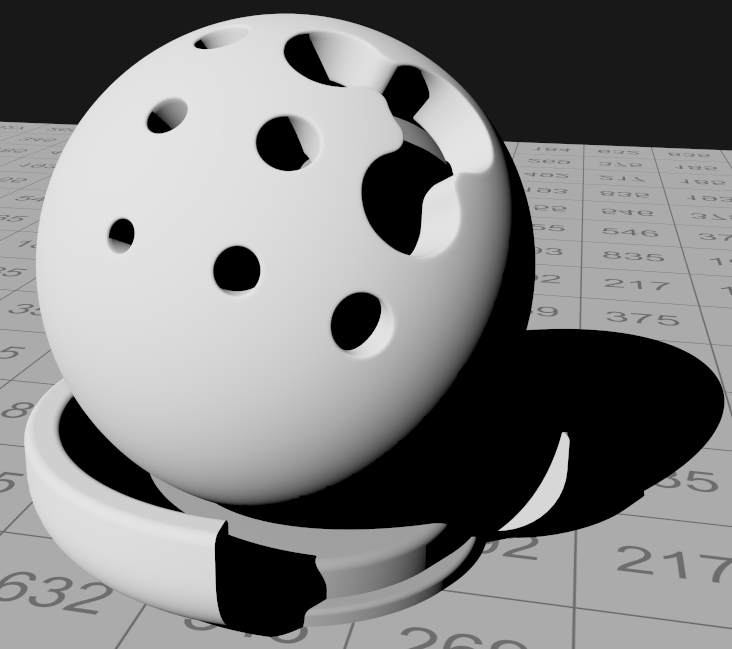
\includegraphics[width=0.95\textwidth]{pic/shaderball-bsdf-0.png}
			\end{subfigure}
			\begin{subfigure}[b]{0.5\textwidth}
				\center
				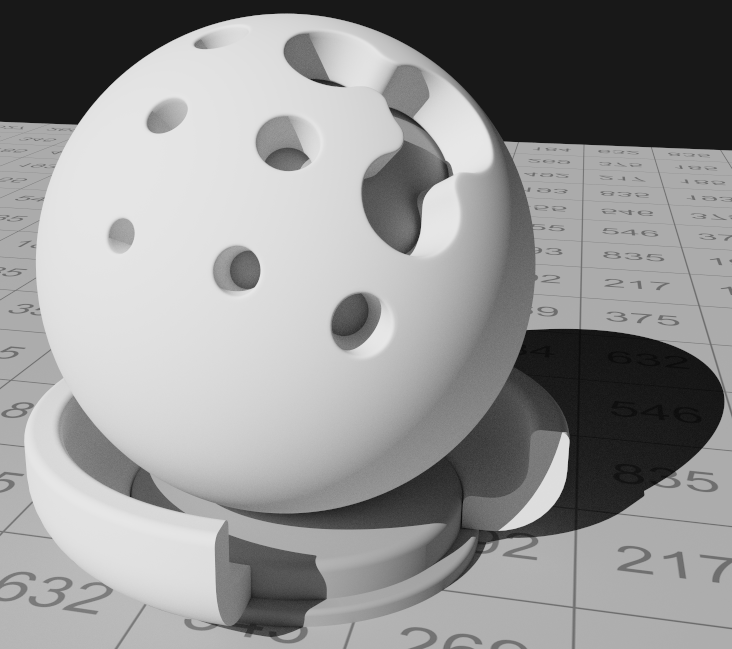
\includegraphics[width=0.95\textwidth]{pic/shaderball-bsdf-10.png}
			\end{subfigure}
			\caption[Unterschied direkter und indirekter Beleuchtung anhand der \enquote{Shaderball}-Szene]{Die Bilder zeigen die gerenderte \enquote{Shaderball}-Szene, beleuchtet durch eine direktionale Lichtquelle. Im linken Bild wurde die Strahldichte der Szene nur durch direkte Beleuchtung ohne die Verwendung einer entsprechenden BSDF berechnet. Im rechten Bild wurde für jedes Material eine lambertsch diffuse Reflexion angenommen. Die Szene wirkt hier wesentlich plastischer und realistischer als im linken Bild.}
			\label{fig:shaderball-bsdf}
		\end{figure}

		Wir wollen nun eine Szene $\Sigma\define(\e{T},\nu,f,E,U)$ und einen Punkt $x\in\e{T}$ betrachten, sodass $f(x,\cdot,\cdot)$ einen Lambertschen Strahler bezüglich $\nu(x)$ darstellt.
		Die Rendergleichung für die Strahldichte $L$ am Punkt $x$ in Richtung $\omega_\m{o}\in\shs{\nu(x)}$ für eine Wellenlänge $\lambda\in(0,\infty)$ lautet dann wie folgt.
		\[
			L(x,\lambda,\omega_\m{o}) = E(x,\lambda,\omega_\m{o}) + \underbrace{\frac{1}{\pi} \integral{\ssp}{}{\mathds{1}_{\shs{\nu(x)}}(\omega) \tilde{L}(x,\lambda,\omega) \abs{\dotp{\nu(x)}{\omega}} }{\sigma(\omega)}}_{\definedby L_\m{r}(x,\lambda,\omega_\m{o})}
		\]
		$L_\m{r}(x,\lambda,\omega_\m{o})$ beschreibt den reflektierten Anteil der Strahldichte.
		Die charakteristische Funktion im Integranden ändert die Integrationsmenge.
		Bezeichnen wir die Irradianz von $L$ durch die Variable $R$, so folgt
		% Folglich gilt für den reflektierten Anteil gerade
		\[
			L_\m{r}(x,\lambda,\omega_\m{o}) = \frac{1}{\pi} \integral{\shs{\nu(x)}}{}{\tilde{L}(x,\lambda,\omega) \dotp{\nu(x)}{\omega}}{\sigma(\omega)} = \frac{R(x,\lambda)}{\pi}
		\]

		Der reflektierte Anteil $L_\m{r}(x,\lambda,\omega_\m{o})$ ergibt sich damit aus der mit $\frac{1}{\pi}$ skalierten Irradianz $R(x,\lambda)$ \cite[S.~785~f]{pbrt2}.
		Insbesondere ist er damit unabhängig von der Richtung $\omega_\m{o}$.
		Das Einsetzen in den übrigen Teil der Gleichung ergibt dann direkt
		\[
			L(x,\lambda,\omega_\m{o}) = E(x,\lambda,\omega_\m{o}) + \frac{1}{\pi}R(x,\lambda)
		\]
		In den meisten Fällen ist $E$ selbst unabhängig von $\omega_\m{o}$ und an vielen Punkten im Raum sogar identisch mit Null.
		Für matte Oberflächen, deren Reflexionsverhalten durch einen Lambertschen Strahler charakterisiert werden kann, reicht es dementsprechend die Irradianz zu betrachten \cite{irr-grad,irradiance-caching}.

		% Wir wollen nun einen Punkt $x$ einer Oberfläche mit Normaler $\mu\in\ssp$ und der BSDF eines lambertschen Strahlers bezüglich $\mu$ betrachten.
		% Dann ergibt sich der Anteil $L_\m{r}$ des reflektierten, aber nicht emittierten Lichtes, am Punkt $x$ in Richtung $\omega_0\in\shs{\mu}$ mit Wellenlänge $\lambda\in(0,\infty)$ aus dem zweiten Term der Rendergleichung.
		% \begin{alignat*}{3}
		% 	L_\m{r}(x,\lambda,\omega_0) &=&&\ \integral{\ssp}{}{ \frac{\mathds{1}_{\shs{\nu}}(\omega_0)}{\pi} \tilde{L}(x,\lambda,\omega) \abs{\dotp{\mu}{\omega}} }{\sigma(\omega)} \\
		% 	&=&&\ \frac{1}{\pi} \integral{\shs{\mu}}{}{\tilde{L}(x,\lambda,\omega) \dotp{\mu}{\omega}}{\sigma(\omega)} = \frac{R(x,\lambda)}{\pi}
		% \end{alignat*}
		% Für den letzten Schritt wurde die Definition der Irradianz bezüglich eines Punktes verwendet.
		% Die reflektierte Strahldichte für einen lambertschen Strahler ist damit unabhängig von der Richtung $\omega_0$ und entspricht gerade der durch $\frac{1}{\pi}$-skalierten Irradianz.
		% Folglich reicht es für ideale diffuse Oberflächen die richtungsunabhängige Irradianz zu betrachten.

		Verwendet man jetzt das Korollar des vorigen Abschnittes, so lässt sich das einfache Modell der Lambertsch diffusen Reflexion zum Beispiel mit einer idealen Reflexion verbinden, wie es in Abbildung \ref{fig:shaderball-bsdf-sum} gezeigt ist.
		Das resultierende Material ist komplexer aufgebaut und beschreibt eine andere Klasse von BSDFs.
		Die Verwendung eines Lambertschen Strahlers kann somit durch Kombination mit anderen BSDF-Modellen auf einen größeren Bereich von Materialarten ausgeweitet werden.
		Mithin ist es in der Praxis in fast allen Szenen nötig, diffuse Reflexionen an den Oberflächen der Objekte auszuwerten.

		\begin{figure}[h]
			\begin{subfigure}[b]{0.5\textwidth}
				\center
				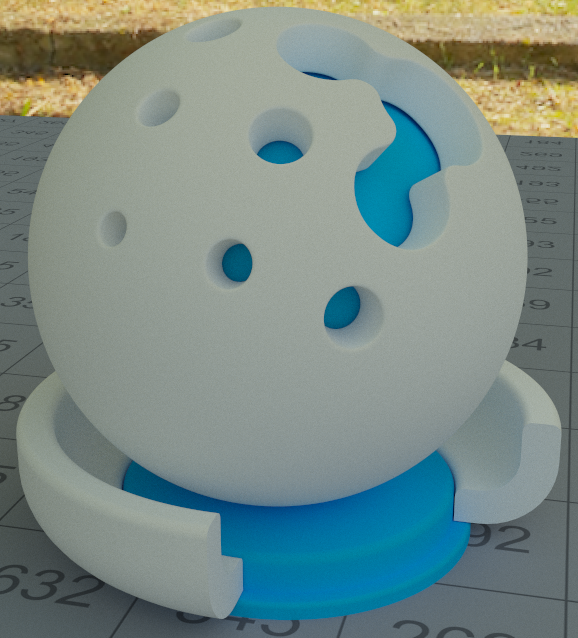
\includegraphics[width=0.95\textwidth]{pic/shaderball-bsdf_sum-diffuse.png}
			\end{subfigure}
			\begin{subfigure}[b]{0.5\textwidth}
				\center
				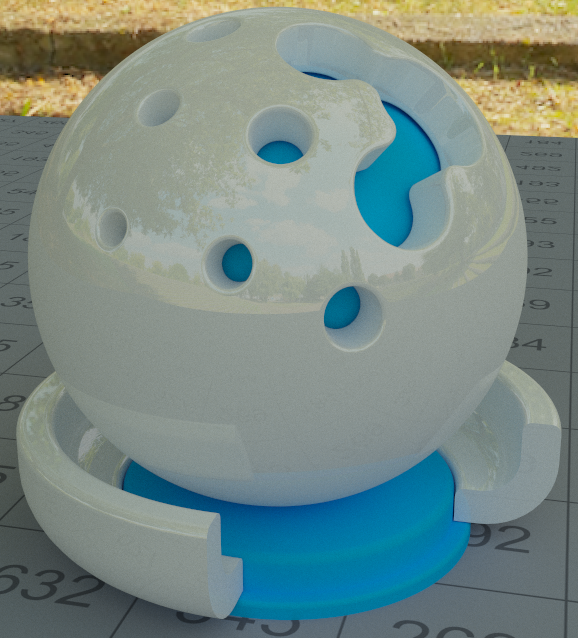
\includegraphics[width=0.95\textwidth]{pic/shaderball-bsdf_sum-specular.png}
			\end{subfigure}
			\caption[Wirkung zusammengesetzter Materialien anhand der \enquote{Shaderball}-Szene]{Die Bilder zeigen die gerenderte \enquote{Shaderball}-Szene, beleuchtet durch eine Umgebungsbeleuchtung. Im linken Bild bestehen die verwendeten BSDFs nur aus der lambertsch diffusen Reflexion. Im rechten Bild wurde das Material der äußeren Körpers zusätzlich mit der BSDF einer idealen Reflexion kombiniert. Das entstehende Material ist kein idealer Spiegel, aber auch kein idealer diffuser Strahler.}
			\label{fig:shaderball-bsdf-sum}
		\end{figure}

		Wir nehmen jetzt an, dass sich die BSDF am Punkt $x$ aus der Kombination eines Lambertschen Strahlers mit Koeffizient $\alpha$ und einer beliebigen BSDF $\tilde{f}(x,\cdot,\cdot)$ mit Koeffizient $\beta$ ergibt.
		Dabei fordern wir, dass $\alpha,\beta\in[0,1]$ und $\alpha +\beta\leq 1$ gilt.
		Das Korollar über die Summe von BSDFs tätigt dann eine klare Aussage über die Form des reflektierten Anteils.
		\[
			L(x,\lambda,\omega_\m{o}) = E(x,\lambda,\omega_\m{o}) + \frac{\alpha}{\pi}R(x,\lambda) + \beta \integral{\ssp}{}{\tilde{f}(x,\omega,\omega_\m{o})\tilde{L}(x,\lambda,\omega)\abs{\dotp{\nu(x)}{\omega}}}{\sigma(\omega)}
		\]

		Diese Form der Rendergleichung für Lambertsche Strahler besitzt für die Verwendung in der Praxis einen Vorteil.
		Die BSDF $\tilde{f}(x,\cdot,\cdot)$ ergibt sich meistens aus stark richtungsabhängigen Anteilen, wie zum Beispiel der idealen Reflexion, der idealen Brechung oder ähnlich glänzenden Materialien.
		Diese Anteile können vergleichsweise gut durch Raytracing beziehungsweise auch Path Tracing gerendert werden.
		Die Berechnung von $R(x,\lambda)$ erfordert jedoch immer eine Integration über die gesamte Hemisphere, bei der jeder erhaltene Wert gleichermaßen gewichtet werden muss.
		Diese Tatsache erschwert die Evaluierung und führt zu entsprechend langen Zeiträumen des Renderings.

		Ein Vorteil der Irradianz besteht jedoch darin, dass sie unabhängig von der betrachteten Richtung ist.
		Die empfangene Strahldichte von $x$ ist konstant, egal von welchem Punkt im Raum aus man $x$ betrachtet.
		Diese Eigenschaft ermöglicht es, $R(x,\lambda)$ vorzuberechnen und am Punkt $x$ zu speichern.
		Jedes Mal, wenn man nun den Punkt $x$ aus einer Richtung $\tilde{\omega}\in\shs{\nu(x)}$ betrachtet, wird das Integral des rechten Teils der Gleichung effizient durch Path Tracing geschätzt. Der Wert $R(x,\lambda)$ kann mit $E(x,\lambda,\tilde{\omega})$ ausgelesen und zum resultierenden Wert hinzugefügt werden.
		Infolgedessen verkürzen sich die benötigten Renderzeiten.
		Da es sich bei $R$ um die Irradianz handelt, wollen wir die zugehörige Datenstruktur, die ihre Werte speichert, \enquote{Irradiance Map} nennen.

		Wir möchten hier bemerken, dass die genannten Eigenschaften nur für die Translation des Beobachtungspunktes gelten.
		Die Änderung der Beleuchtung oder Geometrie führt zu einer neuen Szene $\tilde{\Sigma}$, deren Irradianz $\tilde{R}$ im Allgemeinen nicht $R$ entspricht.
		Die Irradiance Map muss demnach für jede Modifizierung der Szene neu berechnet werden, um die korrekten Werte der Irradianz zu beinhalten.

	% subsection lambertsch_diffuse_materialien_und_die_rendergleichung (end)

	% \subsection{Irradiance Map und Irradiance Cache} % (fold)
	% \label{sub:irradiance_map_und_irradiance_cache}

	% 	In \cite{irradiance-caching} und \cite[S.~783~ff]{pbrt2} wird das Verfahren des sogenannten \enquote{Irradiance Caching} beschrieben.
	% 	Es basiert auf der vorherigen Gleichung und ermöglicht das Zwischenspeichern der Irradianz in einem \enquote{Cache}.
	% 	Dabei werden nur Werte, für die genügend bereits aufgenommene Werte in der Nähe gefunden werden, durch diesen Cache interpoliert.
	% 	Ist dies nicht der Fall, so wird die Irradianz an diesem Punkt neu geschätzt und im Cache abgelegt.
	% 	Der Cache besteht aus einer räumlichen Datenstruktur (engl.: \textit{spatial datastructure}), wie zum Beispiel einem \enquote{Octree}, der die einzelnen Irradianz-Werte mit ihrer Position im Raum unabhängig von der Mesh speichert.
	% 	Dies ermöglicht die Implementierung einer effizienten Suche für die bereits aufgenommenen Werte.

	% 	Irradiance Caching ist damit ein Verfahren, welches in Abhängigkeit des derzeitigen Beobachtungspunktes Werte aufnimmt, speichert und interpoliert.
	% 	Folglich berechnet es nur die Irradianzen an Punkten, die durch den Beobachter gesehen werden.
	% 	Auch die Interpolation kann sich dadurch dem derzeitigen Bildausschnitt anpassen und exaktere Ergebnisse liefern.

	% 	Eines der wichtigsten Probleme besteht darin, dass die Interpolation der aufgenommenen Werte über dem Raum und nicht über der Oberfläche der Szene stattfindet.
	% 	Diese fehlerhafte Interpolation führt in einigen Szenen mit dünnen Wänden zu sogenannten \enquote{light leaks} und anderen Beleuchtungs-Artefakten.
	% 	Weiterhin ist es im Allgemeinen ratsam nur die indirekte Irradianz durch einen Irradiance Cache anzunähern, da sich diese über der Oberfläche nur langsam ändert und gut approximiert werden kann.
	% 	Beleuchtungseffekte, die durch die Umgebungsbeleuchtung oder andere direkte Lichtquellen erzeugt werden, müssen hiernach für jedes Bild neu berechnet werden.

	% 	Ein andere Variante ist die in dieser Arbeit besprochene komplette Vorberechnung einer Irradiance Map.
	% 	Sie speichert die aufgenommenen Werte durch eine passende Datenstruktur auf der Oberfläche der Szene und ermöglicht eine vergleichsweise einfache lokale Interpolation.
	% 	Beispiele finden sich in \cite{course-photon-map,gi-llde,gi-density-estimation}.
	% 	Dies ermöglicht das Speichern der direkten Irradianz und verhindert die Entstehung einiger Beleuchtungsartefakte.
	% 	Allerdings müssen Irradiance Maps auch Werte für Bereiche der Szene speichern, die vom Beobachter aus nicht gesehen werden.
	% 	Dies führt dazu, dass Irradiance Maps im Allgemeinen einen sehr viel höheren Speicherverbrauch aufweisen als Irradiance Caches.

	% subsection irradiance_map_und_irradiance_cache (end)

	\subsection{Schätzung der Irradianz} % (fold)
	\label{sub:schaetzung_der_irradianz}

		In Abschnitt \ref{sub:rendergleichung} wurde erwähnt, dass die meisten Renderverfahren, wie zum Beispiel das hier verwendete Path Tracing, auf der Basis von Zufallsvariablen arbeiten.
		Das Integral in der Rendergleichung wird dabei mithilfe geeigneter Monte-Carlo-Methoden berechnet.
		Aus diesem Grund bildet sich bei den Lösungen der Rendergleichung immer ein gewisses \enquote{Rauschen} (engl.: \textit{noise}) aus.
		In Abbildung \ref{fig:fairy-noise} wird dies an einem Beispiel demonstriert.

		\begin{figure}[h]
			\begin{subfigure}[b]{0.5\textwidth}
				\center
				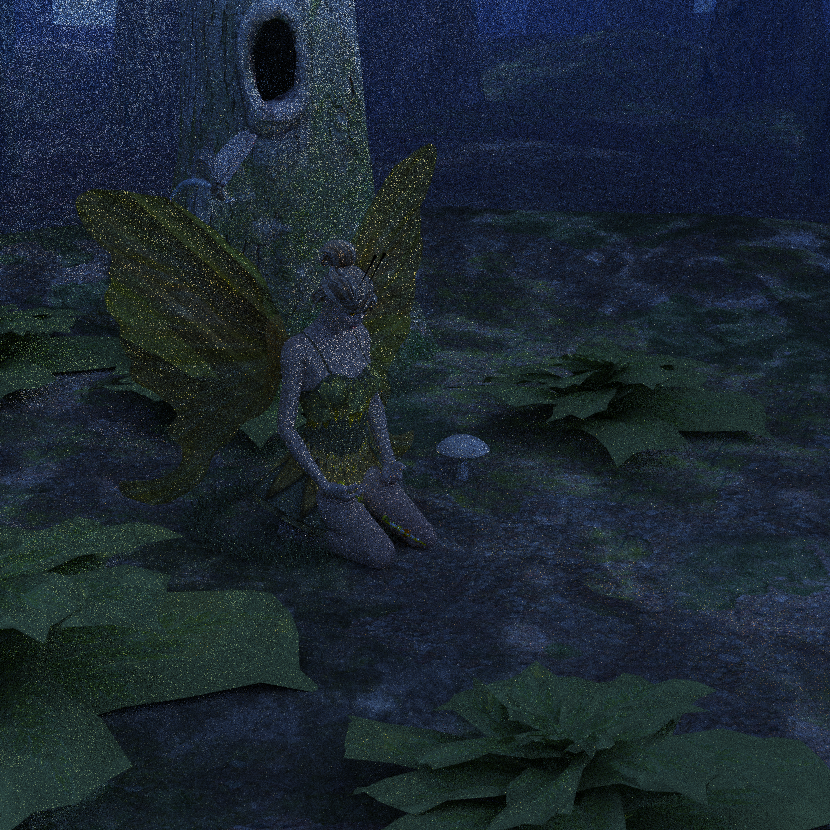
\includegraphics[width=0.95\textwidth]{pic/noise-fairy-high.png}
			\end{subfigure}
			\begin{subfigure}[b]{0.5\textwidth}
				\center
				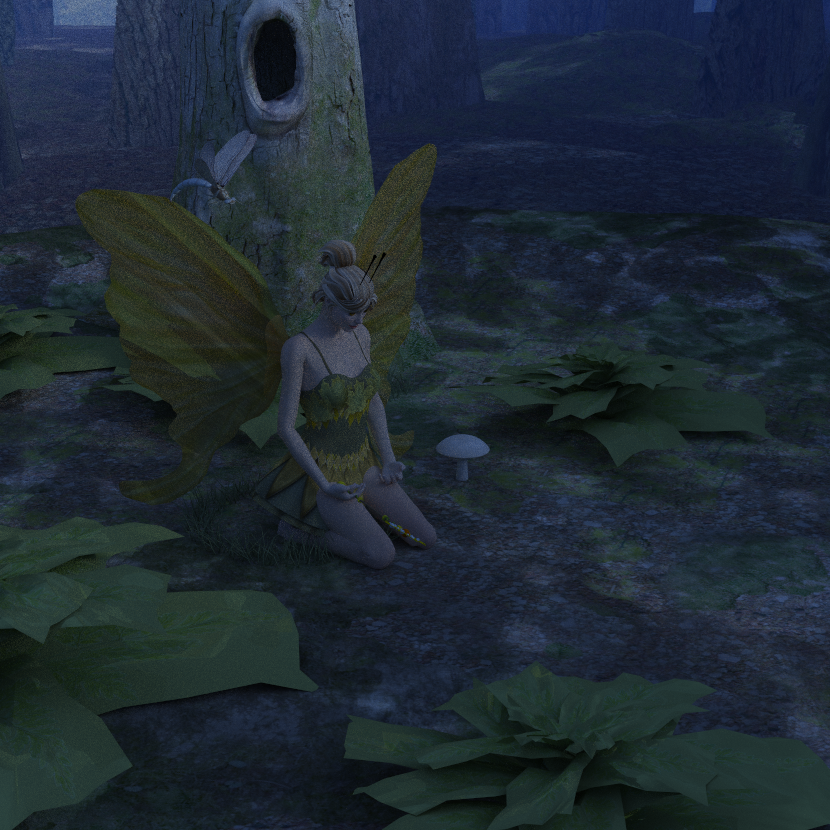
\includegraphics[width=0.95\textwidth]{pic/noise-fairy-low.png}
			\end{subfigure}
			\caption[Rauschen durch Path Tracing anhand der \enquote{Fairy}-Szene]{Die Bilder zeigen die gerenderte \enquote{Fairy}-Szene. Für das linke Bild wurde an jedem sichtbaren Punkt der Szene die Irradianz durch $16$ Messungen ermittelt. Das Resultat beinhaltet noch einen großen Anteil des Rauschens. Im rechten Bild wurden jeweils $1024$ Messungen durchgeführt, wodurch es wesentlich rauschärmer als das Linke ist.}
			\label{fig:fairy-noise}
		\end{figure}

		Möchte man die Irradianz für die Irradiance Map ermitteln, so muss darauf geachtet werden, dass das Rauschen des Endresultates und damit dessen Fehler klein bleibt.
		Erst durch die Beschränkung des Fehlers können gemessene Irradianzen an verschiedenen Punkten interpoliert werden, ohne das Artefakte wie in der späteren Abbildung \ref{subfig:irr-est-rc-shaderball-512} entstehen.

		Für die folgende Betrachtung nehmen wir wieder an, dass eine Szene $\Sigma\define(\e{T},\nu,f,E,U)$ und eine Strahldichte $L$ von $\Sigma$, die der Rendergleichung genügt, gegeben seien.
		Wir bezeichnen $R$ als die Irradianz von $L$ und wählen eine festen Punkt $x\in\e{T}$ und eine feste Wellenlänge $\lambda\in(0,\infty)$.
		Um die Zufälligkeit der Simulation mathematisch zu fassen, verwenden wir einen Wahrscheinlichkeitsraum $(X,\e{X},p)$ und für jedes $\omega\in\ssp$ die folgende Zufallsvariable.
		\[
			\func{\e{L}_\omega}{X}{[0,\infty)},\qquad \expect\e{L}_\omega = \tilde{L}(x,\lambda,\omega)
		\]
		Die Simulation von $\tilde{L}(x,\lambda,\omega)$ durch Path Tracing oder einem ähnlichen Algorithmus entspricht dann der Realisierung $\e{L}_\omega(\xi)$ mit $\xi\in X$.
		Für die Irradianz $R(x,\lambda)$ führen wir einen weiteren Wahrscheinlichkeitsraum $(Y,\e{Y},q)$ ein.
		Seien $n\in\SN$ und unabhängige, identische Zufallsvariablen $\func{w_i}{Y}{\shs{\nu(x)}}$ für alle $i\in\SN,i\leq n$ mit der folgenden zugehörigen Wahrscheinlichkeitsdichte bezüglich $\sigma$ gegeben.
		\[
			\func{\varrho}{\shs{\nu(x)}}{[0,\infty)},\qquad \varrho(\omega)\define\frac{1}{2\pi}
		\]
		Die $w_i$ sind damit für alle $i\in\SN,i\leq n$ auf der Hemisphere $\shs{\nu(x)}$ gleichverteilt.
		Wir sind nun in der Lage weitere Zufallsvariablen $\e{R}_i$ für alle $i\in\SN,i\leq n$ auf dem Produkt-Wahrscheinlichkeitsraum $(X\times Y,\e{X}\otimes\e{Y}, p\otimes q)$ zu definieren, deren Erwartungswert eine Aussage über die Irradianz trifft.
		\[
			\func{\e{R}_i}{X\times Y}{[0,\infty)},\qquad \e{R}_i(\xi,\zeta)\define \e{L}_{w_i(\zeta)}(\xi) \dotp{\nu(x)}{w_i(\zeta)}
		\]
		Die folgende Rechnung zeigt den Zusammenhang des Erwartungswertes von $\e{R}_i$ mit $R(x,\lambda)$ für alle $i\in\SN,i\leq n$.
		\begin{alignat*}{3}
			\expect \e{R}_i &=&&\ \integral{X\times Y}{}{\e{R}_i}{(p\otimes q)} \\
			\text{(Satz von Fubini \cite[S.~175~f]{measure-theory})}\qquad &=&&\ \integral{Y}{}{ \integral{X}{}{ \e{R}_i(\xi,\zeta) }{p(\xi)} }{q(\zeta)} \\
			\text{(Definition $\e{R}_i$)}\qquad &=&&\ \integral{Y}{}{ \integral{X}{}{ \e{L}_{w_i(\zeta)}(\xi) \dotp{\nu(x)}{w_i(\zeta)} }{p(\xi)} }{q(\zeta)} \\
			\text{(Linearität Integral)}\qquad &=&&\ \integral{Y}{}{ \dotp{\nu(x)}{w_i(\zeta)} \integral{X}{}{ \e{L}_{w_i(\zeta)}(\xi)  }{p(\xi)} }{q(\zeta)} \\
			\text{(Definition Erwartungswert)}\qquad&=&&\ \integral{Y}{}{ \dotp{\nu(x)}{w_i(\zeta)}\expect \e{L}_{w_i(\zeta)} }{q(\zeta)} \\
			\text{(Definition $\e{L}_{w_i(\zeta)}$)}\qquad&=&&\ \integral{Y}{}{ \tilde{L}(x,\lambda,w_i(\zeta)) \dotp{\nu(x)}{w_i(\zeta)}}{q(\zeta)} \\
			\text{(Transformation \cite[S.~191~f]{measure-theory})}\qquad &=&&\ \integral{w_i(Y)}{}{ \tilde{L}(x,\lambda,\zeta) \dotp{\nu(x)}{\zeta}}{q_{w_i}(\zeta)} \\
			\text{(Maße mit Dichten \cite[S.~127~f]{measure-theory})}\qquad &=&&\ \integral{\shs{\nu(x)}}{}{\tilde{L}(x,\lambda,\omega)\dotp{\nu(x)}{\omega}\varrho(\omega)}{\sigma(\omega)} \\
			\text{(Definition $\varrho$)}\qquad&=&&\ \frac{1}{2\pi} \integral{\shs{\nu(x)}}{}{\tilde{L}(x,\lambda,\omega)\dotp{\nu(x)}{\omega}}{\sigma(\omega)} \\
			\text{(Definition Irradianz)}\qquad&=&&\ \frac{R(x,\lambda)}{2\pi}
		\end{alignat*}
		Durch diese Äquivalenz erlangen wir die Möglichkeit einen erwartungstreuen Schätzer $\bar{\e{R}}$ der Irradianz $R(x,\lambda)$ zu definieren.
		\[
			\bar{\e{R}} \define \frac{2\pi}{n}\sum_{i=1}^n \e{R}_i
		\]
		Nach Quelle \cite[S.~249~ff]{prob-theory} ergibt sich dann mit einem $i\in\SN,i\leq n$ für den Erwartungswert und die Varianz
		\[
			\expect \bar{\e{R}} = R(x,\lambda),\qquad \var \bar{\e{R}} = \frac{4\pi^2}{n}\var \e{R}_i
		\]
		Wir können also zufällige Richtungen der Hemisphere auswählen und für diese die Strahldichte ermitteln.
		Das arithmetische Mittel sollte dann nach dem \enquote{schwachen Gesetz der großen Zahlen} \cite[S.~254]{prob-theory} für eine steigende Anzahl von Messwerten gegen den Wert der Irradianz konvergieren.
		Es sei hier auch auf die Quellen \cite{kajiya-lte,pbrt3,veach-thesis} verwiesen, die diese Herleitung mithilfe der \enquote{Pfadintegral-Formulierung} der Rendergleichung vollführen.
		Das eben beschriebene Verfahren ist ein typisches Beispiel einer Monte-Carlo-Methode \cite{monte-carlo-method}.
		Die Abbildungen \ref{fig:irr-est-rc-dragon} und \ref{fig:irr-est-rc-shaderball} zeigen es anhand zweier Beispielszenen für verschiedene Sampleanzahlen.

		\begin{figure}[h]
			\begin{subfigure}[t]{0.33\textwidth}
				\center
				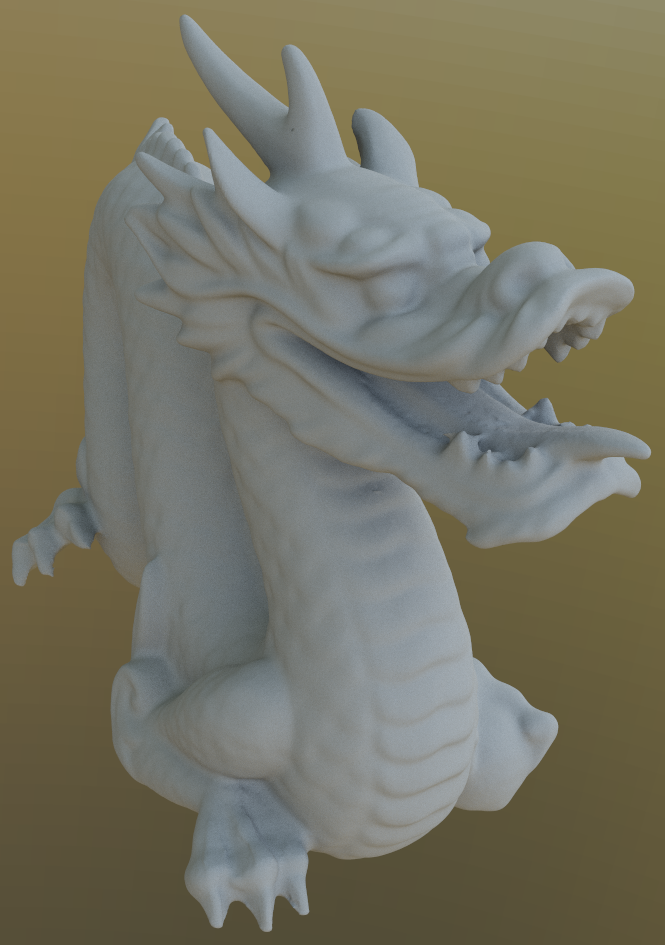
\includegraphics[width=0.95\textwidth]{pic/irr_est-rc-dragon2-ref.png}
				\caption{\parbox[t]{0.5\textwidth}{Path Tracing}}
				\label{subfig:irr-est-rc-dragon-pt}
			\end{subfigure}
			\begin{subfigure}[t]{0.33\textwidth}
				\center
				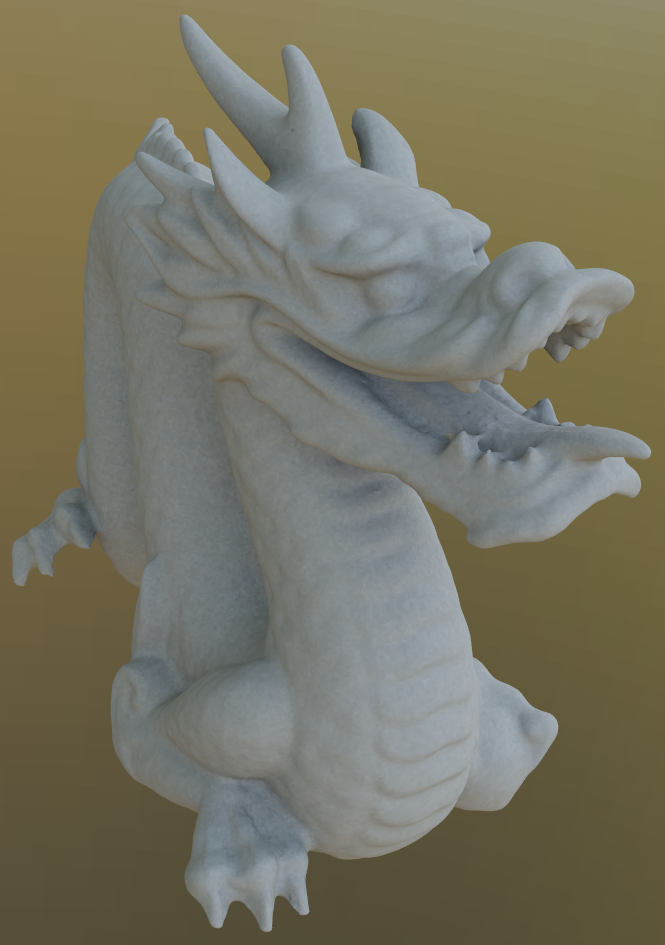
\includegraphics[width=0.95\textwidth]{pic/irr_est-rc-dragon2-s512.png}
				\caption{\parbox[t]{0.5\textwidth}{$512$ Samples \\ $7.32\unit{s}$}}
				\label{subfig:irr-est-rc-dragon-512}
			\end{subfigure}
			\begin{subfigure}[t]{0.33\textwidth}
				\center
				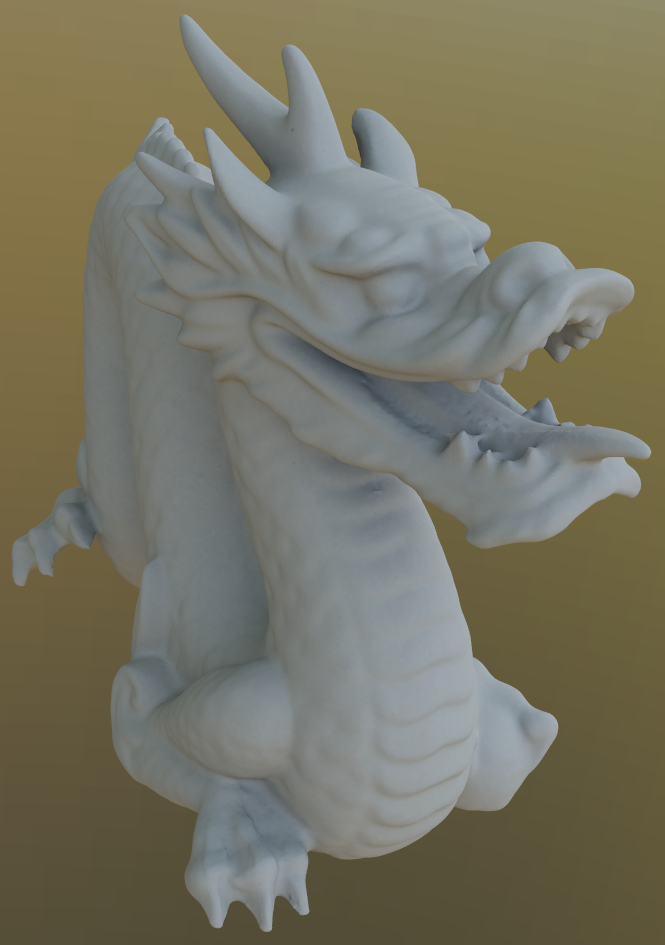
\includegraphics[width=0.95\textwidth]{pic/irr_est-rc-dragon2-s4096.png}
				\caption{\parbox[t]{0.5\textwidth}{$4096$ Samples \\ $56.08\unit{s}$}}
				\label{subfig:irr-est-rc-dragon-4096}
			\end{subfigure}
			\caption[Vertex Lighting anhand der \enquote{Dragon}-Szene]{Die Bilder zeigen die gerenderte \enquote{Dragon}-Szene mit einer schwach variierenden Umgebungsbeleuchtung. \ref{subfig:irr-est-rc-dragon-pt} ist ein durch Path Tracing aufgenommenes Referenzbild. Für \ref{subfig:irr-est-rc-dragon-512} und \ref{subfig:irr-est-rc-dragon-4096} wurden die Irradianzen an den Eckpunkten der Mesh geschätzt und gespeichert. Zwischen den Eckpunkten fand eine lineare Interpolation statt. Die Anzahl der Samples gibt an, wie viele Stichprobenwerte verwendet wurden, um die Irradianz an jedem Punkt zu schätzen. Die Zeit entspricht dabei der Berechnungsdauer. \ref{subfig:irr-est-rc-dragon-4096} weist zum Referenzbild keine Unterschiede auf. In \ref{subfig:irr-est-rc-dragon-512} sind jedoch einige schwache Artefakte in Form von Lichtflecken zu beobachten.}
			\label{fig:irr-est-rc-dragon}
		\end{figure}

		\begin{figure}[h]
			\begin{subfigure}[t]{0.5\textwidth}
				\center
				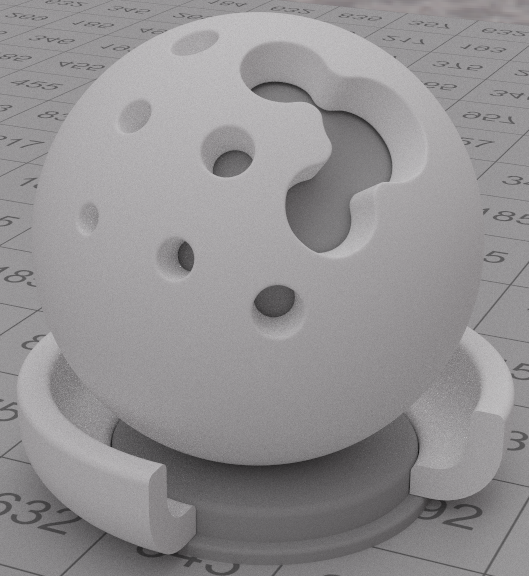
\includegraphics[width=0.95\textwidth]{pic/irr_est-rc-shaderball2-ref.png}
				\caption{\parbox[t]{0.5\textwidth}{Path Tracing}}
			\end{subfigure}
			\begin{subfigure}[t]{0.5\textwidth}
				\center
				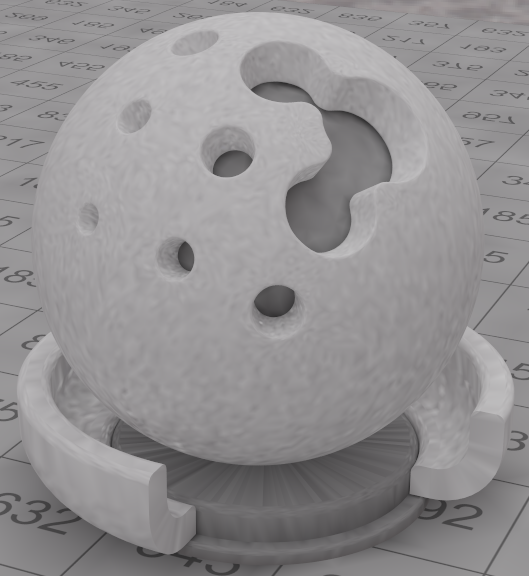
\includegraphics[width=0.95\textwidth]{pic/irr_est-rc-shaderball2-s512.png}
				\caption{\parbox[t]{0.5\textwidth}{$512$ Samples \\ $6.00\unit{s}$}}
				\label{subfig:irr-est-rc-shaderball-512}
			\end{subfigure}
			\medskip \\
			\begin{subfigure}[t]{0.5\textwidth}
				\center
				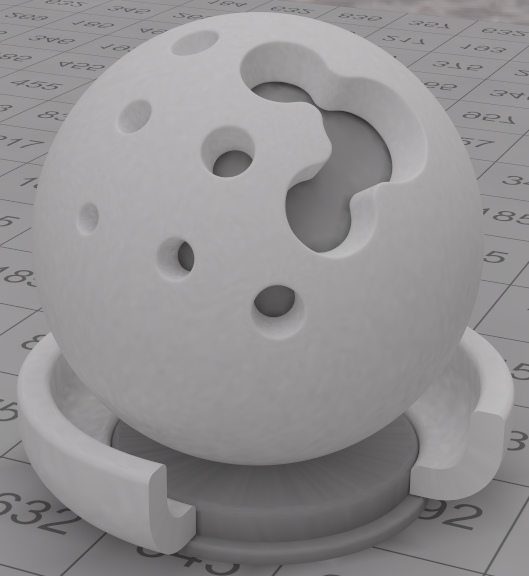
\includegraphics[width=0.95\textwidth]{pic/irr_est-rc-shaderball2-s4096.png}
				\caption{\parbox[t]{0.5\textwidth}{$4096$ Samples \\ $48.85\unit{s}$}}
				\label{subfig:irr-est-rc-shaderball-4096}
			\end{subfigure}
			\begin{subfigure}[t]{0.5\textwidth}
				\center
				
\includegraphics[width=0.95\textwidth]{pic/irr_est-rc-shaderball2-s16384.png}
				\caption{\parbox[t]{0.5\textwidth}{$16384$ Samples \\ $191.22\unit{s}$}}
				\label{subfig:irr-est-rc-shaderball-16384}
			\end{subfigure}
			\caption[Vertex Lighting anhand der \enquote{Shaderball}-Szene]{Die Bilder zeigen die gerenderte \enquote{Shaderball}-Szene mit der \enquote{Uffzi Gallery}-HDR entsprechend der Benennung aus Abbildung \ref{fig:irr-est-rc-dragon}. Die Monte-Carlo-Integration erzeugt in \ref{subfig:irr-est-rc-shaderball-512} mit nur $2^9$ Samples ein fleckiges Muster, welches durch die Verteilung der Zufallsvariable um den Erwartungswert hervorgerufen wird. In \ref{subfig:irr-est-rc-shaderball-4096} und \ref{subfig:irr-est-rc-shaderball-16384} ist erkennbar, dass die Entstehung von Flecken durch eine höhere Sampleanzahl verringert werden kann. Dennoch sind in \ref{subfig:irr-est-rc-shaderball-16384} auch für $2^{14}$ Samples im unteren Stand der Szene noch Flecken sichtbar.}
			\label{fig:irr-est-rc-shaderball}
		\end{figure}

		Die Ergebnisse des Algorithmus varieren stark mit der Szenengeometrie und der gegebenen Umgebungsbeleuchtung.
		Während im Bild \ref{subfig:irr-est-rc-dragon-4096} in der \enquote{Dragon}-Szene mit einer einfachen Umgebungsbeleuchtung bereits nach $4096$ Messungen an einem Punkt kein Unterschied mehr zum Referenzbild \ref{subfig:irr-est-ra-dragon-ref} festgestellt werden kann, sind in der \enquote{Shaderball}-Szene mit der \enquote{Uffzi Gallery}-HDR in Bild \ref{subfig:irr-est-rc-shaderball-16384} mit $16384$ Messungen pro Punkt immer noch fleckige Artefakte zu sehen.

		Eine einfache Erklärung für dieses Phänomen kann durch eine Analyse der Szene gefunden werden.
		Für komplexe Umgebungsbeleuchtungen wie in Anhang \ref{sec:verwendete_hdr_maps} muss im Allgemeinen eine sehr viel höhere Sampleanzahl verwendet werden, um in der Lage zu sein Details, wie zum Beispiel kleine Lichtquellen, aufzulösen und in die Schätzung mit einzubeziehen.
		Weiterhin spielt auch die Konstellation der Dreiecke zum Rest der Szene eine Große Rolle.
		In der \enquote{Dragon}-Szene werden vom Beobachter ausgesendete Strahlen meisten nur ein einziges Mal an der Oberfläche der Mesh reflektiert.
		Nach der Reflexion treffen sie keine weiteren Dreiecke, wodurch im letzten Schritt nur noch die Umgebungsbeleuchtung evaluiert wird.
		Dies verringert die Varianz der gemessenen Irradianz, weil die einfallende Strahldichte für fast alle Richtungen durch die feste Umgebungsbeleuchtung und nicht durch eine Zufallsvariable gegebene ist.
		Im unteren Stand der \enquote{Shaderball}-Szene ist dies nicht mehr der Fall.
		Hier kann es durchaus passieren, dass ein Strahl mehrere Male reflektiert werden muss, um entweder zur Umgebungsbeleuchtung zu gelangen oder durch ein Material absorbiert zu werden.
		Dieser Effekt erhöht die Varianz eines Messpunktes.

		Aus dieser Betrachtung lässt sich schließen, dass die Verringerung der Varianz aller Punkte für beliebige Szenen nur durch extrem hohe Sampleanzahlen möglich ist.
		Eine solche Schätzung für alle Eckpunkte der Szene durchzuführen, wäre zeitraubend und ineffizient.

	% subsection fehlerabschätzung_der_irradianz (end)

	\subsection{Fehler der Irradianzschätzung} % (fold)
	\label{sub:fehler_der_irradianzschaetzung}

		Um die Schätzung der Irradianz effizienter zu gestalten, benötigen wir ein Maß für den Fehler dieser Schätzung.
		Im letzten Abschnitt verwendeten wir hierfür die Varianz der Zufallsvariable.
		Für eine feste vorgegebene Anzahl von Samples zeigte sich diese als ausreichend.
		Möchte man jedoch die Sampleanzahl an verschiedenen Punkten der Oberfläche variieren, so benötigen wir ein Fehlermaß, welches in den Bereichen von Artefakten einen hohen und sonst einen niedrigen Wert besitzt.
		Die Varianz erfüllt diese Eigenschaft nicht, da die Strahldichte und damit auch die Irradianz nach unten aber nicht nach oben beschränkte Funktionen sind.
		Eine Strahldichte mit großem Erwartungswert weist im Allgemeinen einen höhere Varianz als eine Strahldichte mit niedrigem Erwartungswert auf.
		Die weitere Verwendung der Varianz als Fehlermaß würde damit zu extrem genauen Messungen in hellen Bereichen und zu extrem ungenauen Messungen in dunklen Bereichen der Szene führen.
		Die Abbildungen \ref{fig:irr-est-rc-dragon} und \ref{fig:irr-est-rc-shaderball} zeigen jedoch, dass die Entstehung von Artefakten nicht durch die Helligkeit charakterisiert wird.

		Die hier verwendete Altenative ist der sogenannte \enquote{Variationskoeffizient} (engl.: \textit{coefficient of variation} oder \textit{relative standard deviation}, \cite{coeff-of-variation}), der im Folgenden für die Zufallsvariable $\bar{\e{R}}$ des vorigen Abschnittes definiert wird.
		Mithilfe der Zufallsvariablen $\e{R}_i,i\in\SN,i\leq n$ führen wir einen Schätzer $\e{C}$ dieses Koeffizienten ein.
		\[
			\rsd \bar{\e{R}} \define \frac{\sqrt{\var \bar{\e{R}}}}{\expect \bar{\e{R}}},\qquad \e{C} \define \frac{1}{ \bar{\e{R}} } \sqrt{\frac{1}{n(n-1)}\sum_{i=1}^n \curvb{2\pi\e{R}_i - \bar{\e{R}}}^2}
		\]
		$\e{C}$ ist im Allgemeinen nicht erwartungstreu, kann aber für spezielle Verteilungen durch eine Skalierung korrigiert werden \cite{coeff-of-variation}.
		Für hinreichend große $n\in\SN$ ist der eingeführte Bias jedoch vernachlässigbar.
		Um bei der Schätzung des Variationskoeffizienten keine Division durch Null zu erhalten, verwenden wir im Computer eine leicht modifizierte Variante $\tilde{\e{C}}_\varepsilon$ für ein $\varepsilon\in(0,\infty)$, die wir auch als \enquote{relativen Fehler} bezeichnen.
		\[
			\tilde{\e{C}}_\varepsilon \define \frac{1}{ \bar{\e{R}} + \varepsilon } \sqrt{\frac{1}{n(n-1)}\sum_{i=1}^n \curvb{2\pi\e{R}_i - \bar{\e{R}}}^2}
		\]
		Es stellte sich heraus, dass $\varepsilon = 0.0001$ eine gute Wahl ist.
		Die Abbildungen \ref{fig:irr-est-rc-dragon-err} und \ref{fig:irr-est-rc-shaderball-err} zeigen die Szenen der Abbildung \ref{fig:irr-est-rc-dragon} beziehungsweise \ref{fig:irr-est-rc-shaderball}.
		Bei ihnen wird der modifizierte Variationskoeffizient über die Eckpunkte der Meshes interpoliert und dargestellt.
		Ein Vergleich mit den zugehörigen Irradianzbildern zeigt, dass das so erhaltene Fehlermaß gerade in den Bereichen der Artefakte einen hohen Wert besitzt und damit den gestellten Anforderungen Genüge leistet.

		\begin{figure}[h]
			\begin{subfigure}[b]{0.33\textwidth}
				\center
				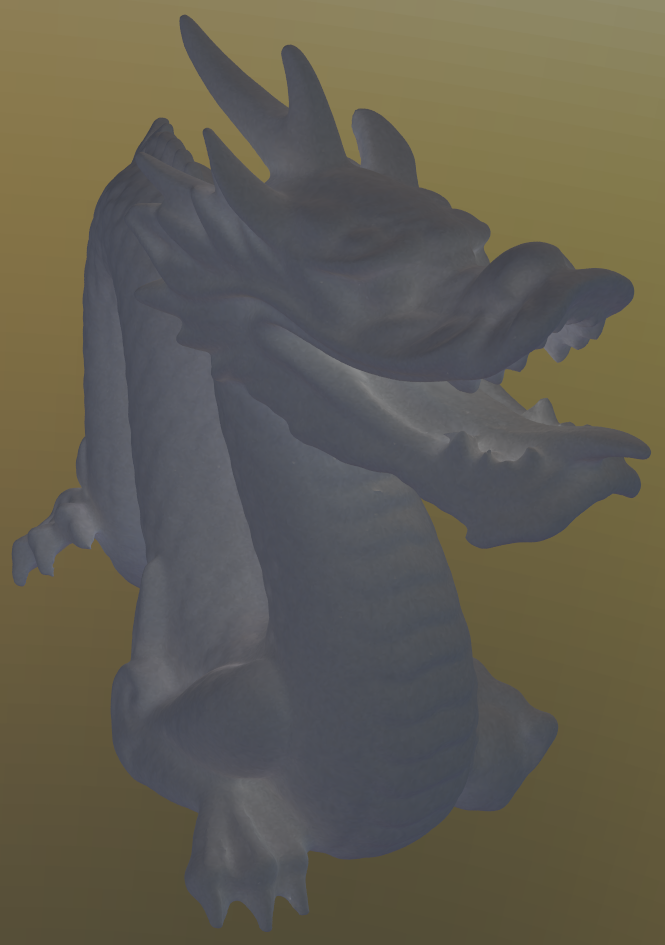
\includegraphics[width=0.95\textwidth]{pic/irr_est-rc-dragon2-s512-err.png}
				\caption{$512$ Samples}
			\end{subfigure}
			\begin{subfigure}[b]{0.33\textwidth}
				\center
				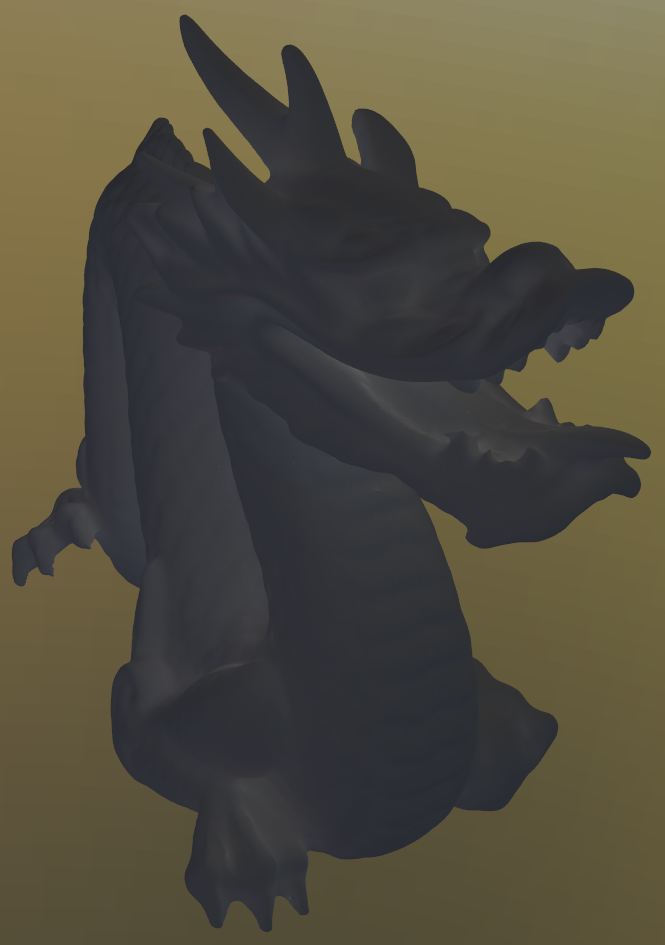
\includegraphics[width=0.95\textwidth]{pic/irr_est-rc-dragon2-s4096-err.png}
				\caption{$4096$ Samples}
			\end{subfigure}
			\begin{subfigure}[b]{0.33\textwidth}
				\center
				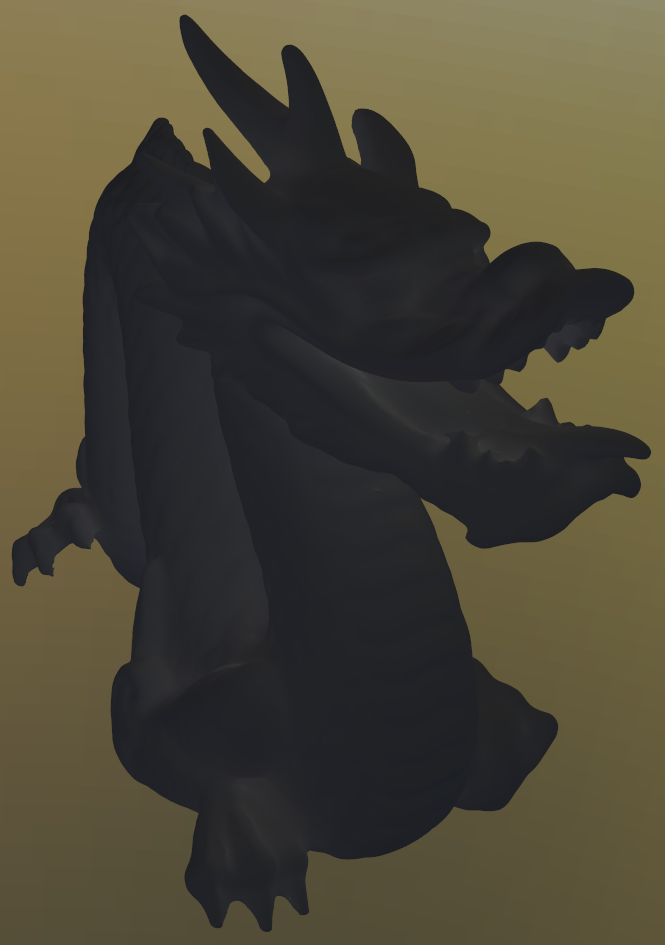
\includegraphics[width=0.95\textwidth]{pic/irr_est-rc-dragon2-s16384-err.png}
				\caption{$16384$ Samples}
			\end{subfigure}
			\caption[Relativer Fehler der \enquote{Dragon}-Szene]{Die Bilder zeigen die \enquote{Dragon}-Szene aus Abbildung \ref{fig:irr-est-rc-dragon} mit den an den Eckpunkten geschätzten modifizierten Variationskoeffizienten. Auch hier findet eine lineare Interpolation zwischen ihnen statt. Eine hellere Farbe bedeutet dabei ein höherer Wert. Deutlich erkennbar ist die Abnahme des Fehlers für größere Sampleanzahlen. Dennoch bleiben auch für $2^{14}$ Samples noch Bereiche, die einen vergleichsweise hohen Fehler aufweisen.}
			\label{fig:irr-est-rc-dragon-err}
		\end{figure}

		\begin{figure}[h]
			\begin{subfigure}[b]{0.33\textwidth}
				\center
				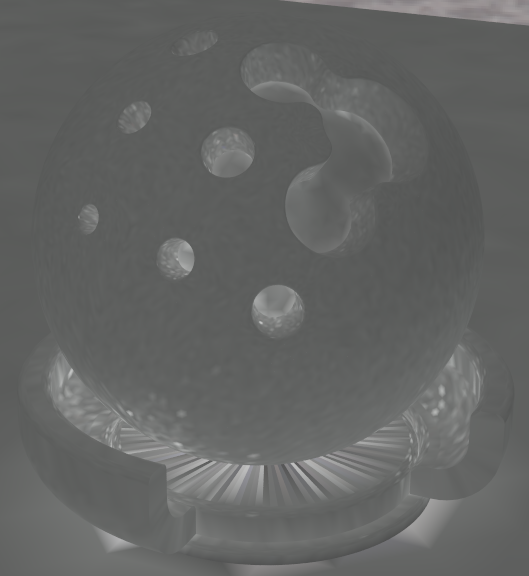
\includegraphics[width=0.95\textwidth]{pic/irr_est-rc-shaderball2-s512-err.png}
				\caption{$512$ Samples}
			\end{subfigure}
			\begin{subfigure}[b]{0.33\textwidth}
				\center
				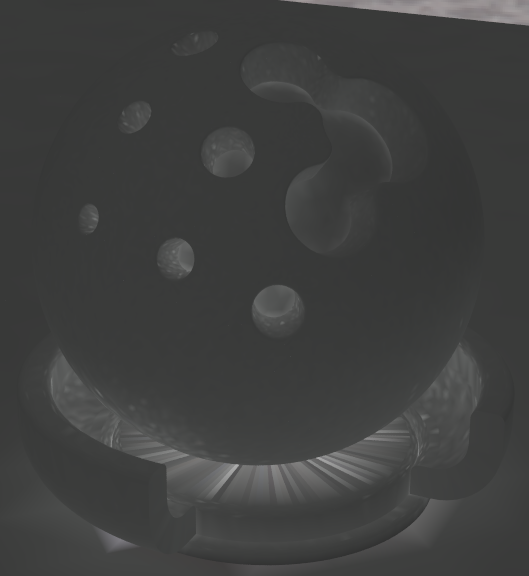
\includegraphics[width=0.95\textwidth]{pic/irr_est-rc-shaderball2-s4096-err.png}
				\caption{$4096$ Samples}
			\end{subfigure}
			\begin{subfigure}[b]{0.33\textwidth}
				\center
				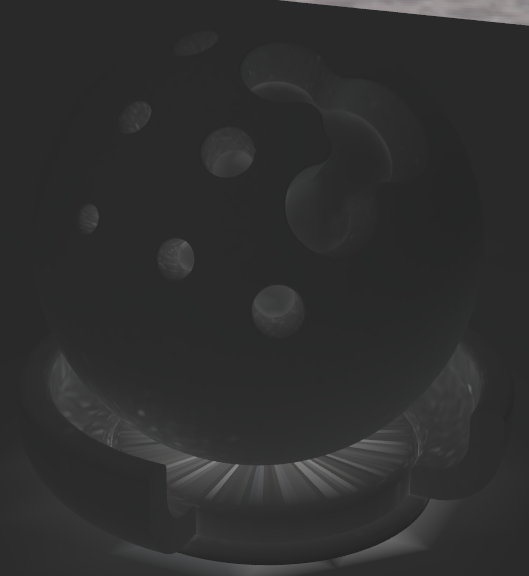
\includegraphics[width=0.95\textwidth]{pic/irr_est-rc-shaderball2-s16384-err.png}
				\caption{$16384$ Samples}
			\end{subfigure}
			\caption[Relativer Fehler der \enquote{Shaderball}-Szene]{Die Bilder zeigen die \enquote{Shaderball}-Szene aus Abbildung \ref{fig:irr-est-rc-shaderball} mit den an den Eckpunkten geschätzten modifizierten Variationskoeffizienten entsprechend der Abbildung \ref{fig:irr-est-rc-dragon-err}. Vor allem Bereiche, die schwach von außen beleuchtet werden oder in Nischen liegen, weisen einen erhöhten Fehler auf. Die regelmäßigen Artefakte im unteren Teil entstehen durch die geringe Auflösung der Mesh.}
			\label{fig:irr-est-rc-shaderball-err}
		\end{figure}

	% subsection fehler_der_irradianzschätzung (end)

	\subsection{Adaptive Schätzung der Irradianz} % (fold)
	\label{sub:adaptive_schaetzung_der_irradianz}

		Das im letzten Abschnitt eingeführte Fehlermaß soll nun verwendet werden, um einen Algorithmus zu formulieren, der die Irradianz eines Punktes effizient durch eine variable Anzahl von Samples schätzen kann.
		Die Idee besteht darin, solange Samples über der Hemisphere aufzunehmen, bis der geschätzte modifizierte Variationskoeffizient kleiner als eine gegebenen Schranke ist.
		Um die Rechenzeit zu beschränken, verwendet man eine maximale Sampleanzahl, nach derer der Algorithmus den geschätzten Wert speichert und terminiert.
		Es gibt aber auch eine vorgeschriebene Mindestanzahl von Samples, die der Algorithmus braucht, um überhaupt den Variationskoeffizienten zu schätzen.
		Der folgende Quelltext implementiert dieses Verfahren durch die Sprache \enquote{C++}.
		Zu beachten ist, dass in der Implementierung selbst die Realisierungen nicht mit $2\pi$ multipliziert werden.
		Diese Vereinfachung ändert jedoch nicht die Funktionsweise.

		\medskip
\begin{tcolorbox}[colframe=black,colbacktitle=white,coltitle=black, attach boxed title to top center={yshift=-2mm},enhanced, titlerule=0.1pt, boxrule=0.5pt, arc=5pt,title=Quelltext:\quad Adaptive Irradianzschätzung]
	\lstinputlisting[style=std,language=c++]{code/est_irr_adap.cpp}
\end{tcolorbox}
\medskip

		Die Ergebnisse des Algorithmus sind in den Abbildungen \ref{fig:irr-est-ra-dragon2}, \ref{fig:irr-est-ra-shaderball2}, \ref{fig:irr-est-ra-shaderball4} und \ref{fig:irr-est-ra-audi3} für verschiedene Szenen und Umgebungsbeleuchtungen gezeigt.
		Weitere Beispiele sind in Anhang \ref{sec:ergebnisse_adaptive_irradianzschaetzung} aufgelistet.
		Lässt man Artefakte, die einer zu geringen Auflösung der Szenengeometrie entspringen, beiseite, so führt die Annäherung der Irradianz in allen Ergebnissen zu einer sehr guten Übereinstimmung mit den zugehörigen Referenzbildern.
		Auch die Berechnungszeit betrug in den meisten Fällen nicht einmal die Hälfte der Zeit des ursprünglichen Verfahrens.
		Zu allen Ergebnissen wurde zudem die Verteilung der Samples angegeben.
		Diese bestätigt die in Abschnitt \ref{sub:schaetzung_der_irradianz} aufgestellten Theorien zur Erklärung der Entstehung von Flecken und ähnlichen Artefakten.
		Die Verwendung einer komplizierten Umgebungsbeleuchtung, wie der \enquote{Ennis-Brown House}-HDR, für die \enquote{Dragon}-Szene in Abbildung \ref{fig:irr-est-ra-dragon2} resultierte in einer wesentlich höheren durchschnittlichen Sampleanzahl als die Verwendung einer schwach variierender Umgebungsbeleuchtung in Abbildung \ref{fig:irr-est-ra-dragon} Anhang \ref{sec:ergebnisse_adaptive_irradianzschaetzung}.
		Auch im unteren Stand oder den oberen Löchern der \enquote{Shaderball}-Szene in den Abbildungen \ref{fig:irr-est-ra-shaderball2} und \ref{fig:irr-est-ra-shaderball4}, in denen Strahlen mehrmals reflektieren, wurden deutlich mehr Samples benötigt als im Rest der gesamten Bilder.
		Dies führt jedoch dazu, dass jegliche vorher sichtbaren zufälligen Artefakte verschwinden.

		\begin{figure}[h]
			\begin{subfigure}[t]{0.33\textwidth}
				\center
				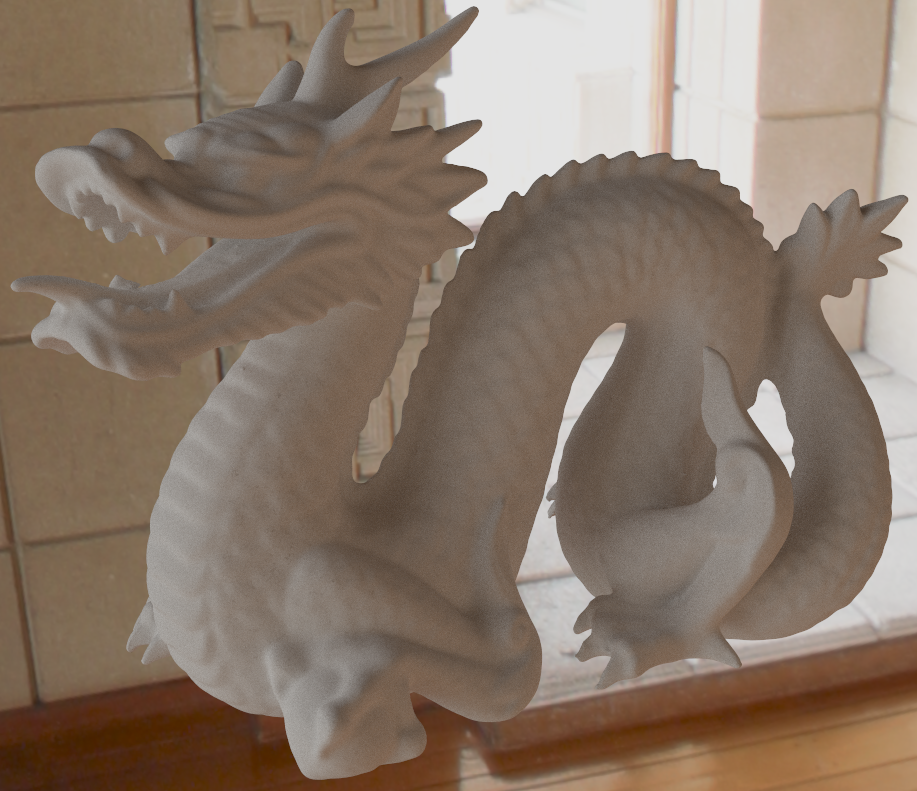
\includegraphics[width=0.95\textwidth]{pic/irr_est-ra-dragon2-ref.png}
				\caption{Path Tracing}
				\label{subfig:irr-est-ra-dragon2-ref}
			\end{subfigure}
			\begin{subfigure}[t]{0.33\textwidth}
				\center
				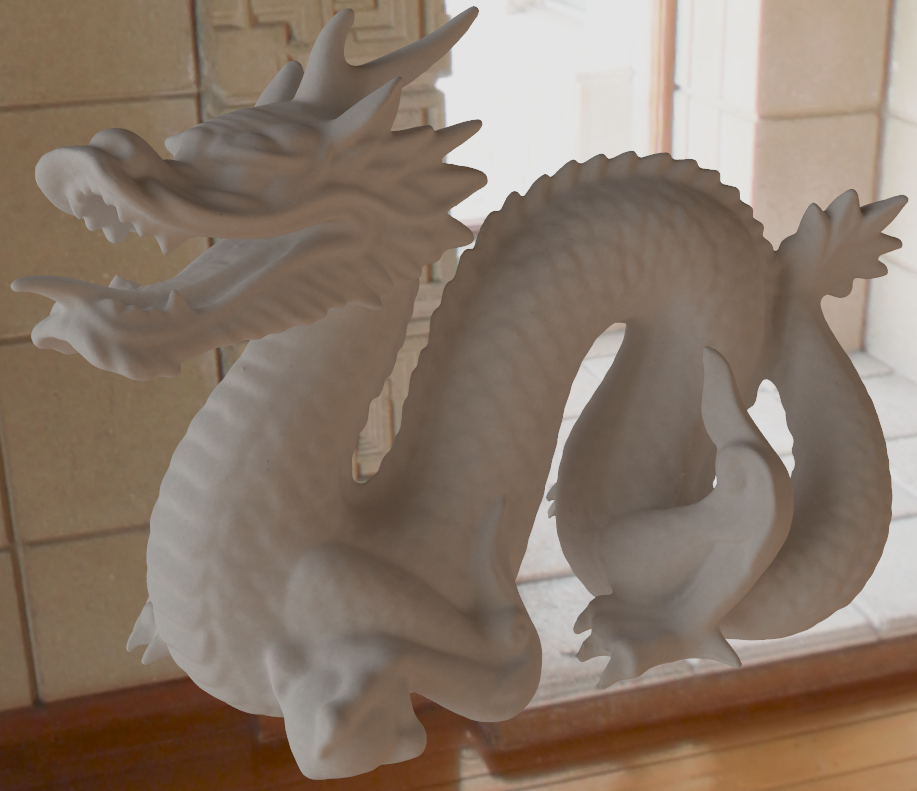
\includegraphics[width=0.95\textwidth]{pic/irr_est-ra-dragon2-irr.png}
				\caption{Irradianz}
				\label{subfig:irr-est-ra-dragon2-irr}
			\end{subfigure}
			\begin{subfigure}[t]{0.33\textwidth}
				\center
				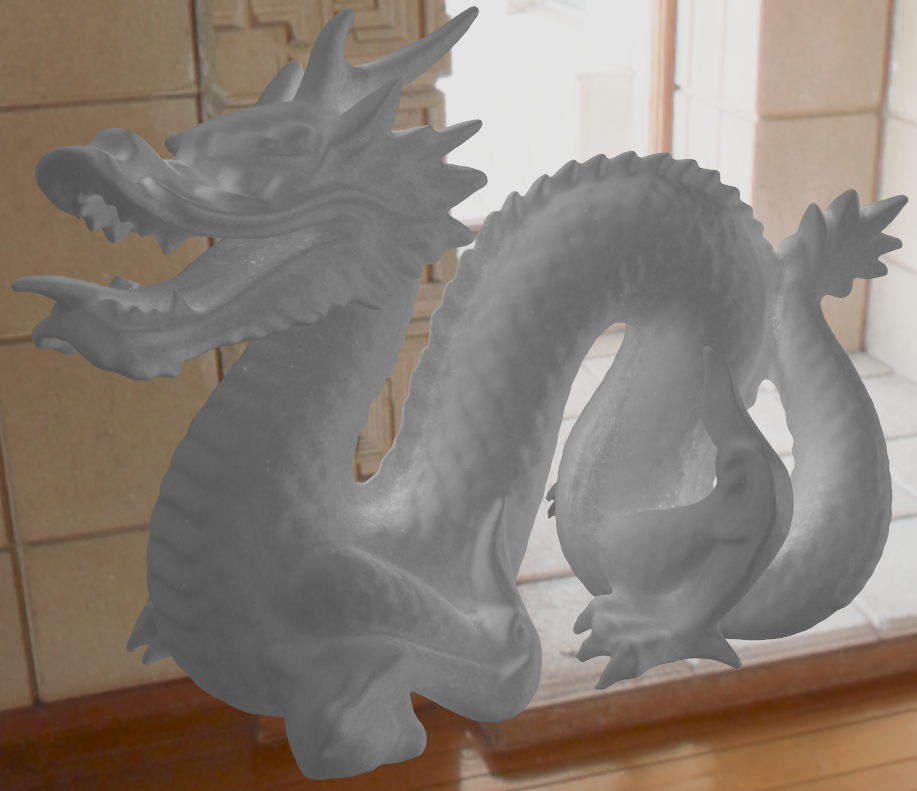
\includegraphics[width=0.95\textwidth]{pic/irr_est-ra-dragon2-scount.png}
				\caption{Sampleanzahl}
				\label{subfig:irr-est-ra-dragon2-scount}
			\end{subfigure}
			\caption[Vertex Lighting anhand der \enquote{Dragon}-Szene mit \enquote{Ennis-Brown House}-HDR]{Die Bilder zeigen die \enquote{Dragon}-Szene mit der \enquote{Ennis-Brown House}-HDR. \ref{subfig:irr-est-ra-dragon2-ref} ist das durch Path Tracing erzeugte Referenzbild. \ref{subfig:irr-est-ra-dragon2-irr} zeigt die an den Eckpunkten adaptiv aufgenommenen Irradianzen mit linearer Interpolation. \ref{subfig:irr-est-ra-dragon2-scount} stellt dabei die zugehörigen Sampleanzahlen dar. Hier bedeutet eine hellere Farbe eine höhere Sampleanzahl. Die Berechnungszeit betrug $559\unit{s}$ mit der maximalen Sampleanzahl $2^{16}$ und einem maximalen relativen Fehler von $3\unit{\%}$.}
			\label{fig:irr-est-ra-dragon2}
		\end{figure}

		\begin{figure}[h]
			\begin{subfigure}[t]{0.33\textwidth}
				\center
				
\includegraphics[width=0.95\textwidth]{pic/irr_est-ra-shaderball2-ref.png}
				\caption{Path Tracing}
			\end{subfigure}
			\begin{subfigure}[t]{0.33\textwidth}
				\center
				
\includegraphics[width=0.95\textwidth]{pic/irr_est-ra-shaderball2-irr.png}
				\caption{Irradianz}
			\end{subfigure}
			\begin{subfigure}[t]{0.33\textwidth}
				\center
				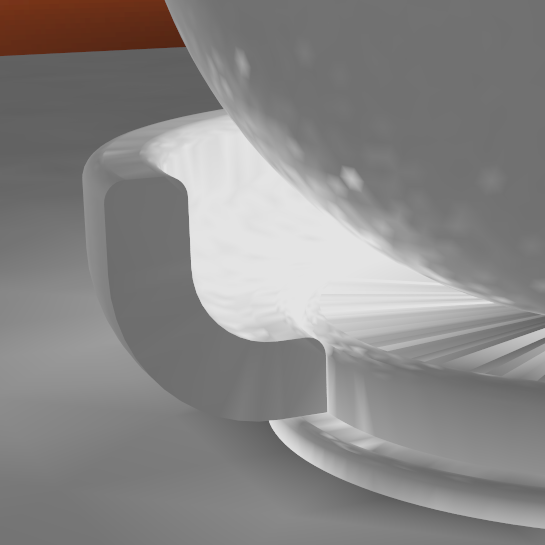
\includegraphics[width=0.95\textwidth]{pic/irr_est-ra-shaderball2-scount.png}
				\caption{Sampleanzahl}
			\end{subfigure}
			\caption[Vertex Lighting anhand der \enquote{Shaderball}-Szene mit \enquote{Ennis-Brown House}-HDR]{Die Bilder zeigen die \enquote{Shaderball}-Szene der Abbildung \ref{fig:irr-est-ra-shaderball} Anhang \ref{sec:ergebnisse_adaptive_irradianzschaetzung} aus einem anderen Blickwinkel unter Verwendung der \enquote{Sky 20}-HDR. Die Benennung ist analog zu Abbildung \ref{fig:irr-est-ra-dragon2}. Die aufgenommenen Irradianzen beinhalten im unteren Stand teilweise weniger Rauschen als das Referenzbild. Die Berechnungszeit betrug $1170\unit{s}$ mit einer maximalen Sampleanzahl $2^{18}$ und einem maximalen relativen Fehler von $1\unit{\%}$.}
			\label{fig:irr-est-ra-shaderball2}
		\end{figure}

		\begin{figure}[h]
			\begin{subfigure}[t]{0.33\textwidth}
				\center
				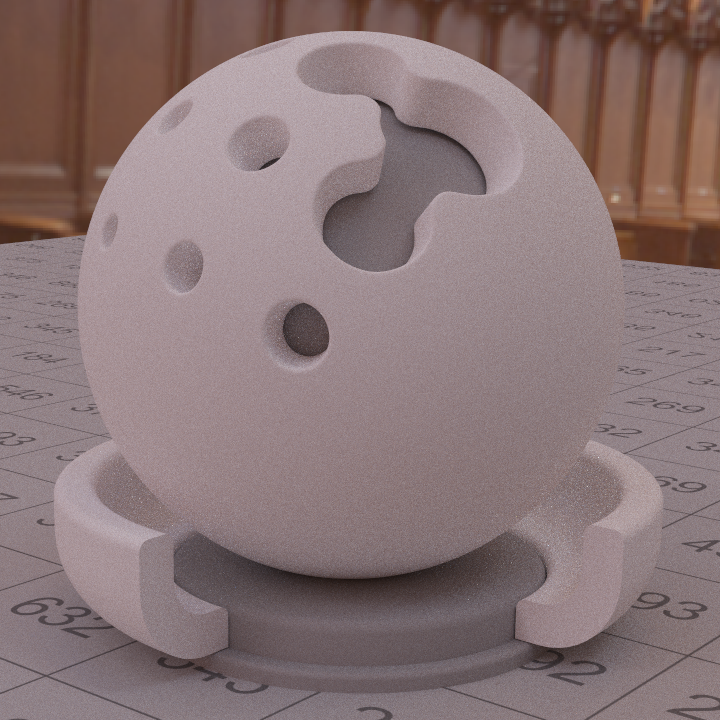
\includegraphics[width=0.95\textwidth]{pic/irr_est-ra-shaderball4-ref.png}
				\caption{Path Tracing}
			\end{subfigure}
			\begin{subfigure}[t]{0.33\textwidth}
				\center
				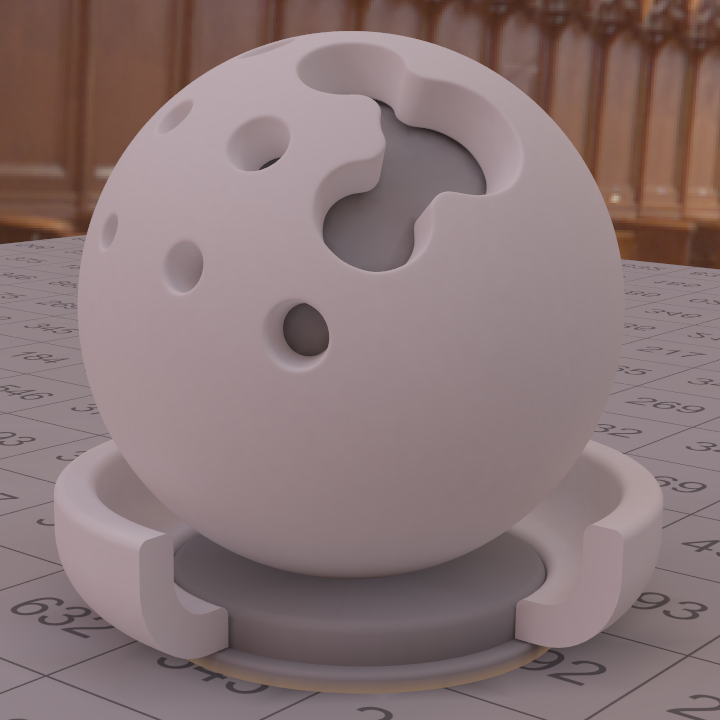
\includegraphics[width=0.95\textwidth]{pic/irr_est-ra-shaderball4-irr.png}
				\caption{Irradianz}
			\end{subfigure}
			\begin{subfigure}[t]{0.33\textwidth}
				\center
				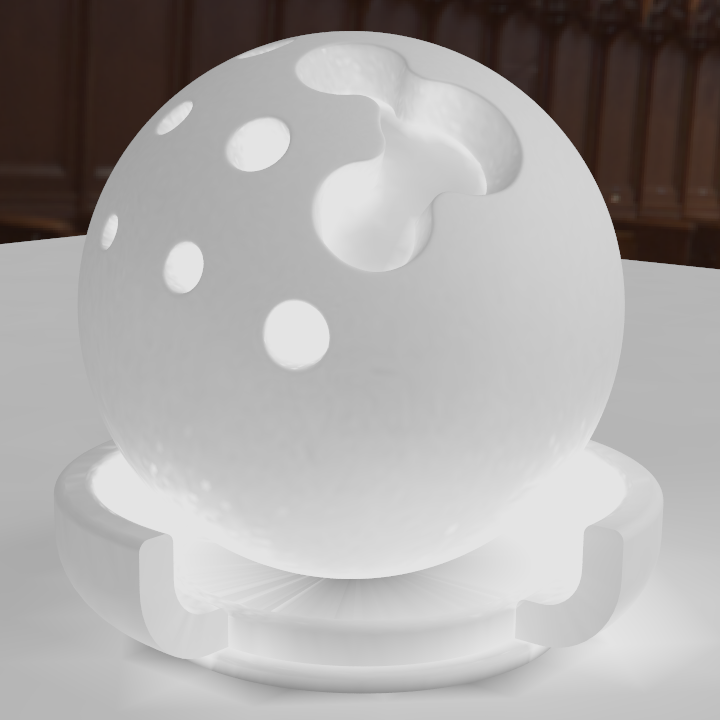
\includegraphics[width=0.95\textwidth]{pic/irr_est-ra-shaderball4-scount.png}
				\caption{Sampleanzahl}
			\end{subfigure}
			\caption[Vertex Lighting anhand der \enquote{Shaderball}-Szene mit \enquote{Ennis-Brown House}-HDR]{Die Bilder zeigen die \enquote{Shaderball}-Szene mit der \enquote{Grace Cathedral}-HDR. Die Benennung ist analog zu Abbildung \ref{fig:irr-est-ra-dragon2}. Die Berechnungszeit betrug $1470\unit{s}$ mit einer maximalen Sampleanzahl von $2^{18}$ und einem maximalen relativen Fehler von $1\unit{\%}$.}
			\label{fig:irr-est-ra-shaderball4}
		\end{figure}

		\begin{figure}[h]
			\begin{subfigure}[t]{0.5\textwidth}
				\center
				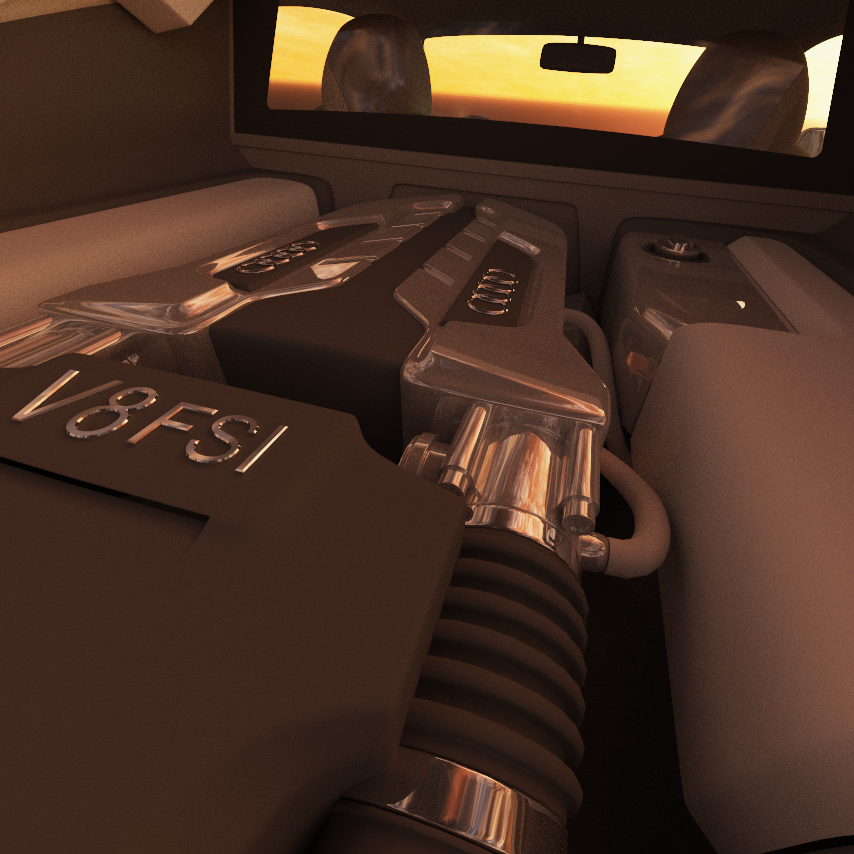
\includegraphics[width=0.95\textwidth]{pic/irr_est-ra-r8_3-ref.png}
				\caption{Path Tracing}
			\end{subfigure}
			\begin{subfigure}[t]{0.5\textwidth}
				\center
				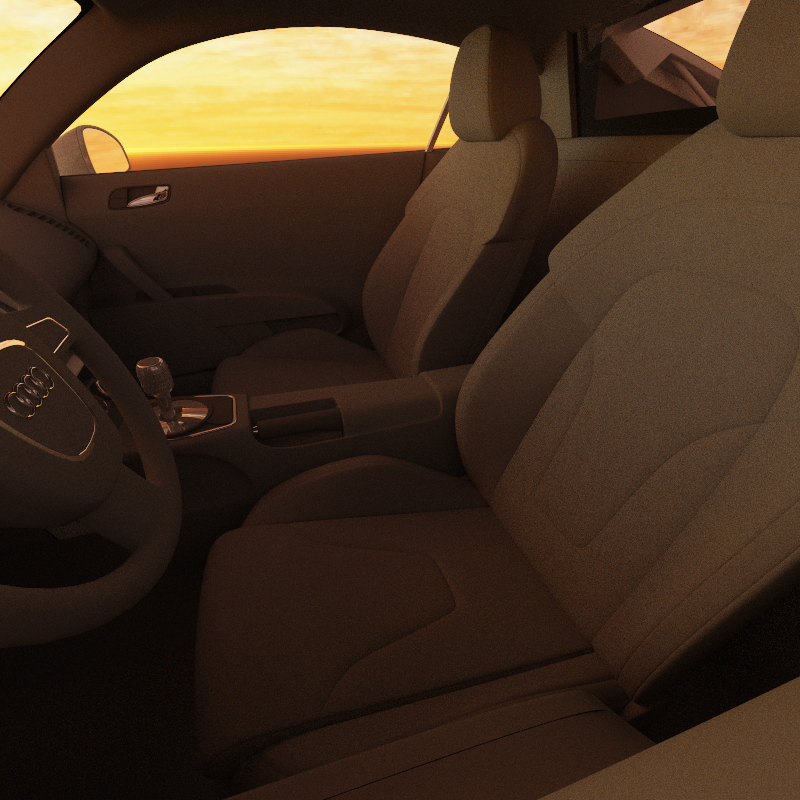
\includegraphics[width=0.95\textwidth]{pic/irr_est-ra-r8_4-ref.png}
				\caption{Path Tracing}
			\end{subfigure}
			\medskip \\
			\begin{subfigure}[t]{0.5\textwidth}
				\center
				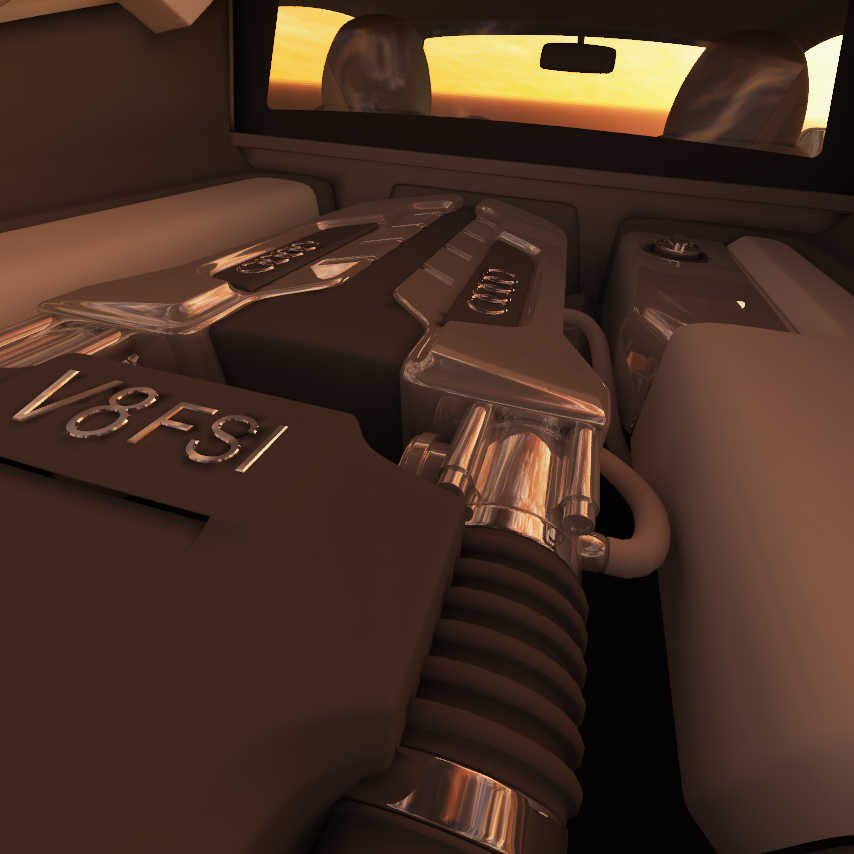
\includegraphics[width=0.95\textwidth]{pic/irr_est-ra-r8_3-irr.png}
				\caption{Irradianz}
			\end{subfigure}
			\begin{subfigure}[t]{0.5\textwidth}
				\center
				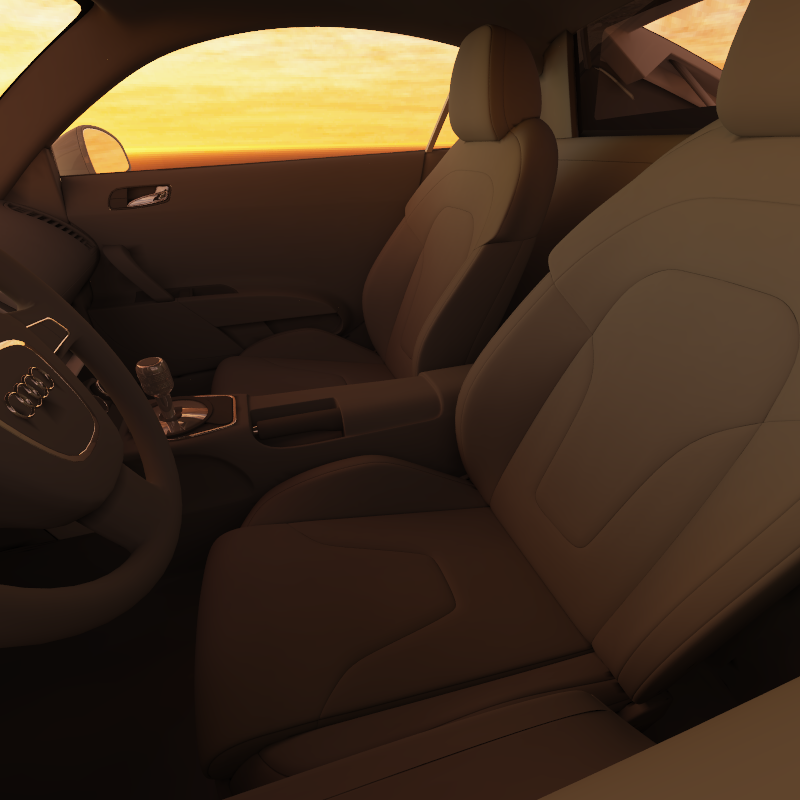
\includegraphics[width=0.95\textwidth]{pic/irr_est-ra-r8_4-irr.png}
				\caption{Irradianz}
			\end{subfigure}
			\medskip \\
			\begin{subfigure}[t]{0.5\textwidth}
				\center
				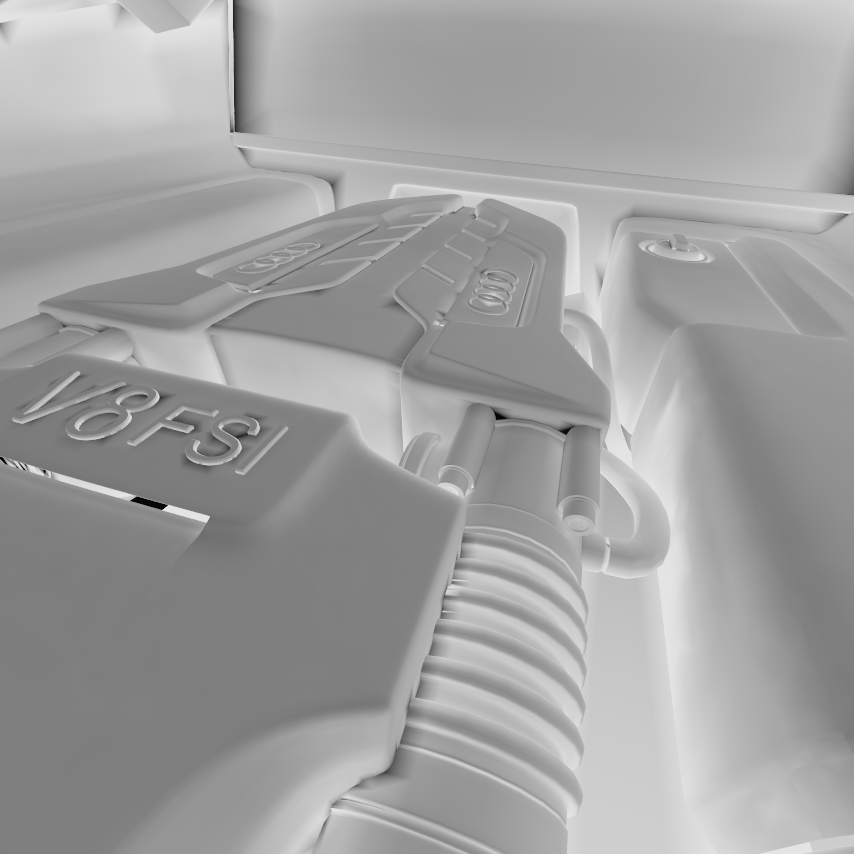
\includegraphics[width=0.95\textwidth]{pic/irr_est-ra-r8_3-scount.png}
				\caption{Sampleanzahl}
			\end{subfigure}
			\begin{subfigure}[t]{0.5\textwidth}
				\center
				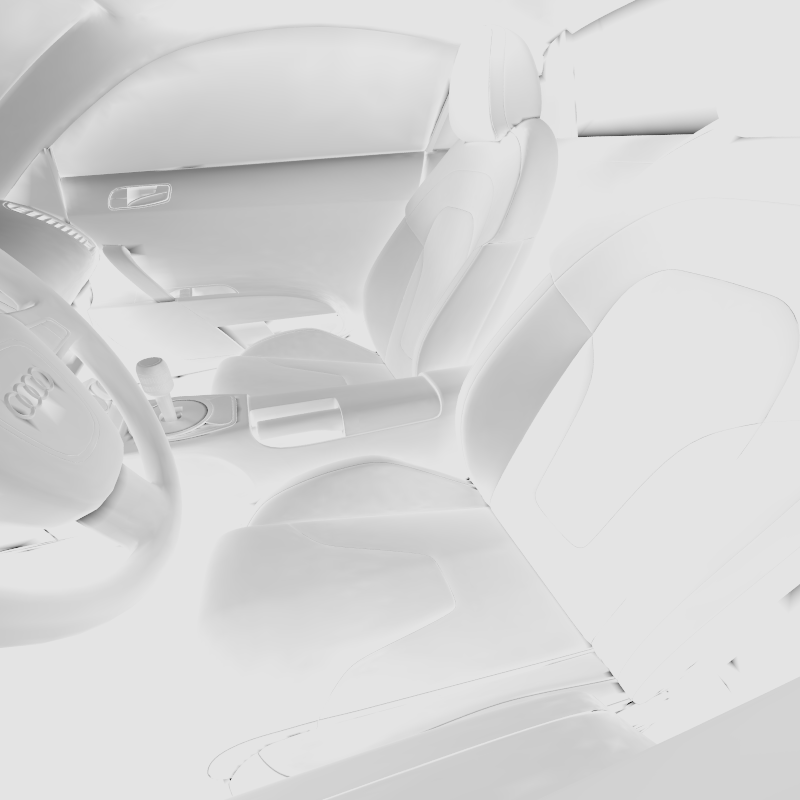
\includegraphics[width=0.95\textwidth]{pic/irr_est-ra-r8_4-scount.png}
				\caption{Sampleanzahl}
			\end{subfigure}
			\caption[Vertex Lighting anhand der \enquote{Audi R8}-Szene mit \enquote{Sky 20}-HDR]{Die Bilder zeigen die \enquote{Audi R8}-Szene mit der \enquote{Sky 20}-HDR aus zwei unterschiedlichen Blickwinkeln und einer analogen Benennung zu Abbildung \ref{fig:irr-est-ra-dragon2}. Die Berechnungszeit betrug $17.8\unit{h}$ mit einer maximalen Sampleanzahl $2^{18}$ und einem maximalen relativen Fehler von $1\unit{\%}$. Zu beachten ist, dass die adaptive Irradianzschätzung im Inneren der Szene zu einem rauschfreien Resultat führt.}
			\label{fig:irr-est-ra-audi3}
		\end{figure}

		\FloatBarrier

		Ein komplexeres Beispiel anhand der \enquote{Audi R8}-Szene mit der \enquote{Sky 20}-HDR ist in den Abbildungen \ref{fig:irr-est-ra-audi} und \ref{fig:irr-est-ra-audi2} aus Anhang \ref{sec:ergebnisse_adaptive_irradianzschaetzung} und der Abbildung \ref{fig:irr-est-ra-audi3} zu sehen.
		In der Szene wurden diverse zusammengesetzte BSDFs verwendet um einen realistischeren Eindruck zu vermitteln.
		Für die Scheiben und Scheinwerfer wurde ein Glas-Material verwendet, welches die ideale Brechung von Licht für einen gegebenen Brechungsindex zulässt.
		Vor allem im Inneren der Szene in Abbildung \ref{fig:irr-est-ra-audi3} werden extrem viele Strahlen benötigt.
		In diesen Bereichen kann Licht, welches durch die Umgebungsbeleuchtung ausgesendet wird, nur durch die Transmission von Strahlen an den Glasscheiben eingesammelt werden.
		Da aber auch die Transmission als zufälliger Prozess betrachtet wird, ist die Wahrscheinlichkeit, Licht einzusammeln, äußerst gering.
		Die Folge ist, dass sowohl bei der Irradianzschätzung als auch beim Path Tracing mit sehr hohen relativen Fehlern beziehungsweise starkem Rauschen zu rechnen ist.
		Außerhalb der Szene werden eigentlich nur in den Radkästen und unter dem Auto viele Samples benötigt.
		Ein Großteil der Strahlen trifft nach einer Reflexion direkt auf die Umgebungsbeleuchtung, was wieder einen sehr kleinen relativen Fehler zur Folge hat.

		In allen Messungen konnten durch die Verwendung einer oberen relativen Fehlerschranke von $1\unit{\%}$ und einer maximalen Sampleanzahl von $2^{18}$ die zufälligen Fehler der Schätzung stark verringert werden, sodass das menschliche Auge nicht mehr in der Lage war, diese zu erkennen.
		Auch in sehr dunklen Bereichen war die Verwendung von $256$ Samples als Mindestanzahl vollkommen ausreichend.
		Dennoch sind die Berechnungszeiten in allen Ergebnissen viel größer als die Darstellungszeit des Path Tracing Bildes.
		Eine der Ursachen besteht in der Konvergenzordnung des adaptiven Irradianzschätzers.
		Aus Abschnitt \ref{sub:schaetzung_der_irradianz} ist bekannt, dass sich die Varianz dieses Schätzers aus der folgenden Gleichung mit den zuvor eingeführten Variablen für ein $i\in\SN,i\leq n$ ergibt.
		\[
			\var \bar{\e{R}} = \frac{4\pi^2}{n}\var \e{R}_i
		\]
		Die Standardabweichung und damit auch der relative Fehler des Schätzers konvergieren also nur mit der Laufzeitkomplexität $\Theta_n\curvb{\frac{1}{\sqrt{n}}}$ gegen Null.
		Die Halbierung des Fehlers fordert dementsprechend viermal so viele Samples wie zuvor \cite[S.~39~f]{veach-thesis}.
		Um diese Eigenschaft zu verbessern, wurde eine Vielzahl von Varianzreduktionsmethoden entwickelt, wie zum Beispiel \enquote{Stratified Sampling} \cite[S.~432~ff]{pbrt3}, \enquote{Importance Sampling} \cite[S.~794~ff]{pbrt3} und \enquote{Quasi-Monte-Carlo Integration} \cite{quasi-monte-carlo}.
		Viele dieser Verfahren sind zwar auf eine konstante Sampleanzahl ausgelegt, könnten aber durch Modifikationen für eine adaptive Irradianzschätzung verwendet werden.
		Zum Beispiel würde es sich bei Stratified Sampling als Vorteil erweisen eine konstante Anzahl von \enquote{Stratas} zu verwenden und durch eine unabhängige Stichprobe deren Gewichtung zu ermitteln.
		Die Schätzung der Irradianz mithilfe dieser Gewichte würde zu einer geringeren benötigten Gesamtsampleanzahl führen und so das Verfahren beschleunigen.
		Eine weitere Herangehensweise ist die Abänderung der Interpolation zwischen Punkten.
		Anstatt für jeden Punkt ein lineares Verfahren zu verwenden, könnte man einen komplexeren Filter oder auch Kern (engl.: \textit{kernel}) durch Berechnung der Faltung mit den geschätzten Irradianzwerten benutzen \cite[S.~402~ff]{pbrt3}.
		Dies könnte dazu führen, dass sich zufällige Fehler nicht durch sichtbare kleine Flecken auf der Oberfläche auswirken, sondern durch nicht-wahrnehmbare Farbverläufe.
		Damit wäre man nicht gezwungen eine obere Fehlerschranke von $1\unit{\%}$ zu verwenden und demnach würde auch dieser Ansatz das Verfahren beschleunigen.
		Eine Änderung der Interpolation würde den Algorithmus der adaptiven Schätzung jedoch nicht abändern.

	% subsection adaptive_schätzung_der_irradianz (end)

% section schätzung_der_irradianz (end)